%%%%%%%%%%%%%%%%%%%%%%%%%%%%%%%%%%%%%%%%
%% MCM/ICM LaTeX Template %%
%% 2025 MCM/ICM %%
%%%%%%%%%%%%%%%%%%%%%%%%%%%%%%%%%%%%%%%%

% Format
\documentclass[12pt]{article}
\usepackage{geometry}
\geometry{left=1in, right=0.75in, top=1in, bottom=1in}

\newcommand{\Problem}{F}
\newcommand{\Team}{2500434}

\usepackage{newtxtext}
\usepackage{amsmath,amssymb,amsthm}
\usepackage{newtxmath}
\usepackage[pdftex]{graphicx}
\usepackage{subfig}
\usepackage{xcolor}
\usepackage{fancyhdr}
\usepackage{enumitem}
\usepackage{titlesec}
\usepackage{tocloft}
\usepackage{lastpage}
\usepackage[hidelinks]{hyperref}

% Page Settings
\pagestyle{fancy}
\lhead{Team \# \Team}
\rhead{Page \thepage\ of \pageref{LastPage}}

% Mathematical env.
\newtheorem{theorem}{Theorem}
\newtheorem{corollary}[theorem]{Corollary}
\newtheorem{lemma}[theorem]{Lemma}
\newtheorem{definition}{Definition}

% Format of table of contents
\renewcommand{\cftsecleader}{\cftdotfill{\cftdotsep}}
\renewcommand{\contentsname}{\begin{center} INDEX \end{center}}

% Format of subsection and subsubsection
\titleformat{\section}{\bfseries\raggedright\Large}{\thesection}{1em}{}
\titleformat{\subsection}{\bfseries\raggedright}{\thesubsection}{1em}{}{}
\titleformat{\subsubsection}{\bfseries}{\hspace*{2em}\thesubsubsection}{1em}{}{}

% CoverPage Design
\begin{document}
\graphicspath{{.}}  % Place the graphic file in the same directory as the main document
\DeclareGraphicsExtensions{.pdf, .jpg, .tif, .png}
\thispagestyle{empty}
\vspace*{-16ex}
\centerline{
\begin{tabular}{*3{c}}
	\parbox[t]{0.3\linewidth}{\begin{center}\textbf{Problem Chosen}\\ \Large \textcolor{red}{\Problem}\end{center}}
	& \parbox[t]{0.3\linewidth}{\begin{center}\textbf{2025\\ MCM/ICM\\ Summary Sheet}\end{center}}
	& \parbox[t]{0.3\linewidth}{\begin{center}\textbf{Team Control Number}\\ \Large \textcolor{red}{\Team}\end{center}}	\\
	\hline
\end{tabular}}

% TODO: Summary
% 1. 12-point Times New Roman font ;
% 2. pdf naming format: 2500434.pdf ;
% 3. No name of school, advisor, or team members .
\begin{center}
Hello Summary!
\end{center}

\newpage
\tableofcontents
\newpage

\section{Introduction}\label{sec:introduction}
%1
\subsection{Background}\label{subsec:background} %1.1
	In the digital age, the speed and scale of global connectivity have reached unprecedented heights.
	However, with technological advancements, \textbf{cybercrime} has also become increasingly complex and diverse.
	These crimes pose significant threats and challenges to personal privacy, corporate assets, national security, and social stability.
	The transnational and covert nature of cybercrime makes it difficult to address effectively.
	Attackers often exploit legal differences and technical vulnerabilities across countries to evade accountability.
	Additionally, many businesses and institutions, concerned about their reputation and commercial interests,
	often choose \textbf{not to publicly report} cyberattacks, opting instead to pay ransoms or handle incidents privately.
	This further exacerbates the hidden nature of cybercrime.
	Developed countries, with their highly digitized economic and social structures, are often prime targets for cybercrime, while
	developing countries face their own unique challenges.

	To address this global challenge, countries have introduced national cybersecurity \textbf{policies}
	aimed at enhancing their defensive capabilities through legal, technical, and organizational cooperation.
	The \textbf{effectiveness} of these policies varies significantly across nations, and these differences may be closely related to factors
	such as policy design, enforcement, technological infrastructure, education levels, economic development, and internet penetration rates.
	In this context, understanding which factors make certain countries' cybersecurity policies more effective has become a critical issue.
	By analyzing the global distribution of cybercrime, national cybersecurity policies, and their outcomes,
	we can identify which policies and laws are particularly effective in preventing, prosecuting, and mitigating cybercrime.
	This data-driven analysis not only helps countries improve their cybersecurity policies
	but also provides valuable insights for global cybersecurity cooperation.
\subsection{Restatement of the problem}\label{subsec:restatement-of-the-problem} %1.2
	We are required to identify patterns
	that can inform the data-driven development and refinement of national cybersecurity policies and laws,
	which focused on those that have demonstrated effectiveness.
	Our goal is to develop a theory explaining what constitutes a strong national cybersecurity policy and then
	support it with a data-driven analysis.

	Several key aspects are listed below:
	\begin{itemize}
		\item Patterns in cybercrime distributed worldwide.
		\item Assessment to effectiveness of National Cybersecurity Policies.
		\item Correlation between national demographics and our distribution analysis.
	\end{itemize}
\subsection{Analysis of problems}\label{subsec:analysis-of-problems} %1.3
	We have divided each problem into several different steps:
	\subsubsection[]{Cybercrime distribution across the world} %1.3.1
		\begin{itemize}
			\item Process the JSON files published on VCDB .
			\item Use GCI as the primary indicator to assess countries with disproportionately high levels of cybercrime.
			\item Group countries based on GCI Tier measure, and
				visually represent the distribution of cybercrime in each group using heatmaps.
		\end{itemize}
	\subsubsection[]{Effective policy or law analytical approach} %1.3.2
		\begin{itemize}
			\item Identify a representative country from each of the T1 to T5 national clusters and
				collect cybersecurity-related policies enacted by these countries.
			\item Plot time-series line graphs depicting the trends of cybercrime over time and
				analyze which policies have been effective in curbing criminal activities.
			\item Conduct a targeted analysis of specific policy models' effectiveness in certain countries,
				focusing on particular indicators.
			\item Integrate temporal factors and national contexts to comprehensively evaluate the impact of policies.
		\end{itemize}
	\subsubsection[]{National demographics correlation} %1.3.3
		\begin{itemize}
			\item TODO % TODO: fill the blank 1.3.3
		\end{itemize} %1

\section{Symbol and Assumptions}\label{sec:symbol-and-assumptions}
%! Author = Yilin
%! Date = 2025/1/27

\subsection{Symbol Description}\label{subsec:symbol-description} %2.1
\begin{tabular}{cl}
    \hline
    \textbf{Symbol} & \textbf{Description} \\
    \hline
    $D_i$                     & Cybercrime distribution in each country. \\
    $P_i$                     & Population of each country. \\
    $y$                       & Transformed value using \( y = \log(1 + x) \). \\
    $\mathbb{E}[Crime_t]$     & Poisson regression model predicted value. \\
    $\beta_0$                 & Intercept term. \\
    $\beta_1,\beta_2,\beta_3$ & Regression coefficients. \\
    $Bill_{t-k}$              & Lagged variable. \\
    $K$                       & Greatest lagged number. \\
    $\rho$                    & Spearman rank correlation coefficient \\
    $d_i$                     & Difference between the ranks of each pair of observations \\
    $n$                       & Number of observations \\
    \hline
\end{tabular}

\bigskip

\noindent
\begin{tabular}{cl}
    \hline
    \textbf{Abbreviation} & \textbf{Full Form} \\
    \hline
    GCI   & Global Cybersecurity Index\cite{gci-2024} \\
    VERIS & the Vocabulary for Event Recording and Incident Sharing\cite{veris} \\
    VCDB  & the VERIS Community Database\cite{vcdb} \\
    GDP   & Gross Domestic Product \\
    VIF   & Variance Inflation Factor \\
    \hline
\end{tabular}
\subsection{Assumptions}\label{subsec:assumptions} %2.2
\begin{itemize}
    \item Countries with a population below 5\% are excluded from the consideration of cybercrime distribution because
        a small change of number could bring a significant difference to statistical analysis.
    \item In the statistical analysis of the global distribution of cybercrime,
        factors such as national population growth, internet access, wealth levels, and education levels
        are assumed to have no significant impact on the quantitative distribution of cybercrime incidents.
        This study hypothesizes that the distribution of cybercrime can be more intuitively understood by focusing solely on the number of incidents,
        independent of these socio-economic variables.
        This assumption is based on all available data recorded since the inception of cybercrime statistics,
        aiming to isolate the distribution patterns of cybercrime from other potential influencing factors.
    \item The impact of newly enacted laws or policies on cybercrime is not instantaneous;
        there is a time lag before their effects become evident.
\end{itemize}
 %2

\section{A Data-Driven Model for Global Cybercrime Hotspot Mapping}
\label{sec:a-data-driven-model-for-global-cybercrime-hotspot-mapping}
Despite the continuous evolution of national cybercrime since the inception of data collection,
along with changes in policies, legal frameworks, and population demographics,
we can create a global cybercrime hotspot map by leveraging crime data recorded by VERIS over the years.
This not only facilitates the analysis of cybercrime volumes by country
but also allows for fitting the data against policy and population variables to assess their influence on cybercrime trends.
\subsection{Cybercrime distribution across the globe}\label{subsec:Building-the-hotspot-map} %3.1
	We made use of a world-wide map to represent all cybercrime occurred around the world.
	In the map, the color filled in each country represents the total number of cybercrime incidents recorded since the beginning of the statistics.
	The color gradient, ranging from dark blue to dark red, corresponds to eight severity levels (1 to 8).
	Countries marked in blue indicate a low frequency of cybercrime incidents, while those marked in red represent a high density of such incidents.
	For instance, the United States, where the VERIS concept was first proposed, has the highest number of recorded incidents (7,236),
	whereas many other countries have only 1 or 2 recorded incidents.
	To address this significant disparity in data distribution, we applied a logarithmic transformation to the data using the formula
	\[ y=\log(1+x) \]
	where x here represents $D_i$.
	This transformation was implemented using the function
	\[ np.log1p() \]
	in Python to ensure computational precision and stability, particularly for small values.
	The final results are visualized in Figure 1.
	\begin{figure}[htbp]
		\centering
		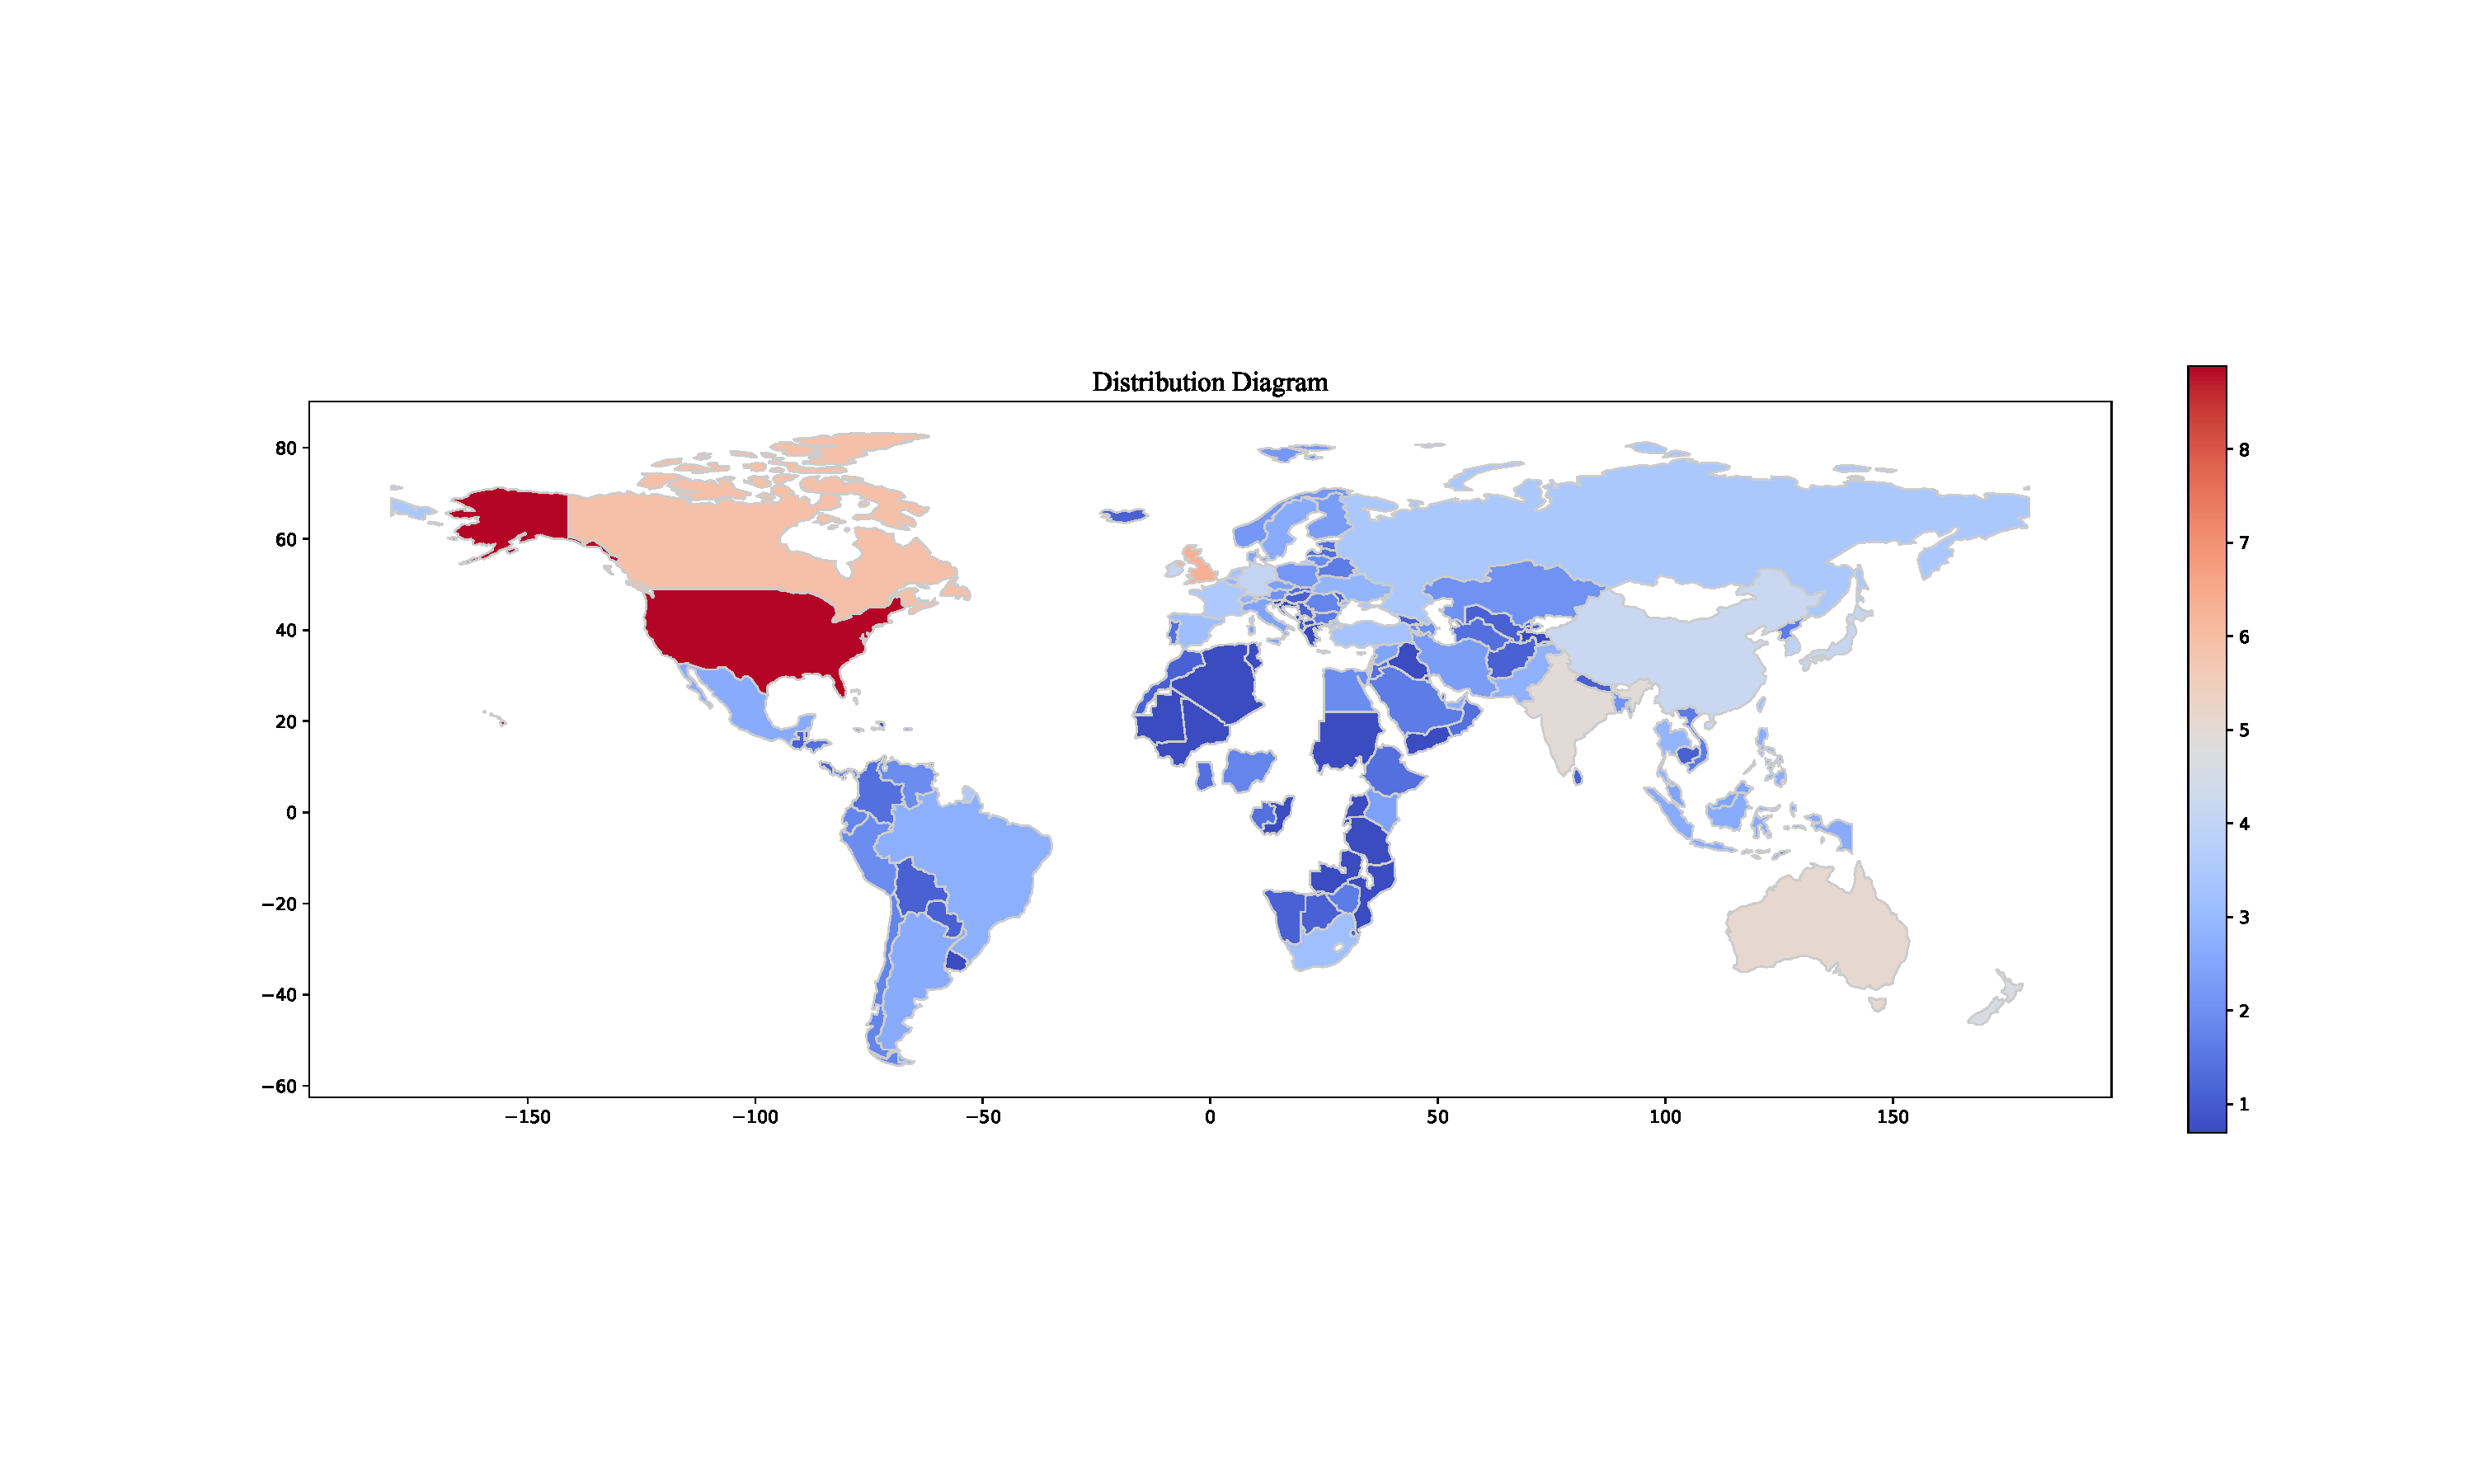
\includegraphics[width=1\linewidth]{../rsrc/distributions/Crime_distribution}
		\caption{Crime distribution}\label{fig:crime-distribution}
	\end{figure}
\subsection{High-prevalence regions}\label{subsec:high-prevalence-regions} %3.2
	We obtained population data $P_i$ for various countries over recent decades from the World Bank Group's website\cite{population}.
	Simultaneously, we processed data from the VCDB to tabulate the annual number of cybercrime incidents $D_i$ for each country from 2000 to 2025.
	However, due to discrepancies in the specific countries reported by the World Bank Group and those listed in the VCDB,
	we had to exclude certain countries to ensure that only those appearing in both datasets were retained.
	Ultimately, 109 countries were included in the model.
	To represent the average number of cybercrime incidents per capita,
	we calculated the ratio $D_i/P_i$ for each year from 2000 to 2025.
	Since the resulting values were too small for practical analysis,
	we scaled them by a factor of $10^{8}$ to express the data as the number of cybercrime incidents per 100 million people,
	denoted as $hmD/P_i$:
	\[ hmD/P_i = \frac{D_i}{P_i} \times 10^{8} \]

	According to the GCI (Global Cybersecurity Index) standards, countries are classified into five tiers, denoted as T1 to T5.
	We used this classification as the basis for K-means clustering analysis,
	dividing the 109 countries into five groups based on the percentiles published on the GCI website:
	the top 10\%, the next 20\%, the following 25\%, the subsequent 25\%, and the bottom 20\%.
	For each group, the annual average of $hmD/P_i$ (the number of cybercrime incidents per 100 million people) was calculated.
	To visualize the results, we constructed a 3D clustering heatmap of cybercrime trends,
	where the x-axis represents the five tiers (T1 to T5),
	the y-axis represents the time span from 2000 to 2025,
	and the z-axis represents the average $hmD/P_i$ values.
	This visualization is presented in Figure\ref{fig:3D_with_Spaced_Projection}.
	\begin{figure}[htbp]
		\centering
		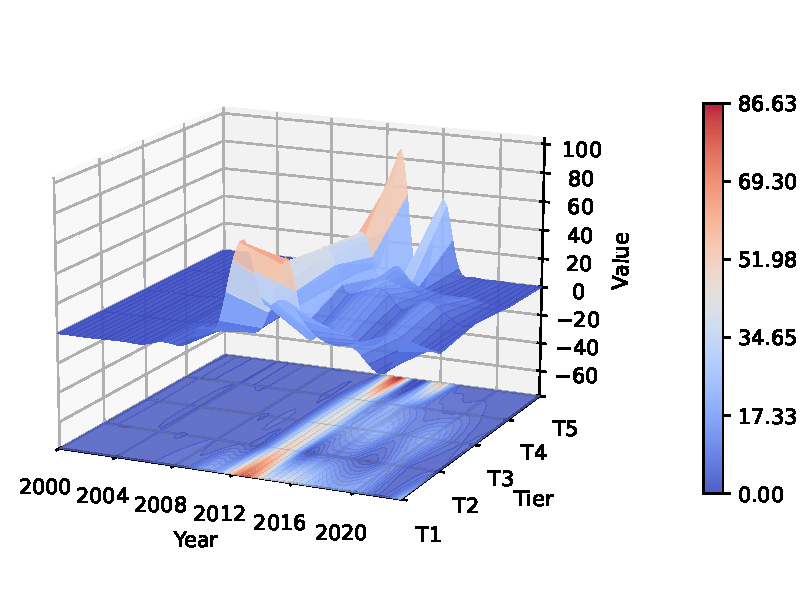
\includegraphics[width=0.8\linewidth]{../rsrc/distributions/3D_with_Spaced_Projection}
		\caption{3D with Spaced Projection}\label{fig:3D_with_Spaced_Projection}
	\end{figure}
\subsection{Other Cybercrime Incidents}\label{subsec:other-cybercrime-incedents} % 3.3
	Using additional data obtained from the VCDB,
	we constructed heatmaps on a global scale based on the number of successful cybercrimes, thwarted cybercrimes, and reported cybercrimes, respectively.
	Due to the disproportionately high volume of data from the United States,
	we applied the same logarithmic transformation (\( y = \log(1 + x) \)) as in Figure~\ref{fig:crime-distribution} for consistency,
	where $x$ represents successful attacks, thwarted attacks, and reported attacks,
	resulting in the three sub-figures presented in Figure\ref{fig:other-cybercrime-incidents}.

	In sub-figure (a), the number of successful attacks closely aligns with the total number of attacks in most countries.
	For instance, the United States recorded 7,189 successful attacks out of 7,236 total attacks,
	yielding a success rate of \( \frac{7189}{7236} \approx 99.35\% \).
	Similarly, the United Kingdom reported 569 successful attacks out of 574 total attacks,
	with a success rate of \( \frac{569}{574} \approx 99.13\% \).

	In contrast, countries with lower attack volumes did not show significant differences between the total number of attacks and the number of successful attacks,
	indicating that almost every attempted attack was successful.

	In sub-figure (b), only the United States and Canada reported thwarted attack cases, with 6 and 2 instances, respectively.

	In sub-figure (c), the number of successfully reported attacks and the number of countries involved were significantly higher than in sub-figure (b).
	This suggests that while many attacks were successful, a portion of them were detected and reported.
	\begin{figure}[htbp]
		\centering
		\subfloat[Successful Cybercrime Incidents]{
			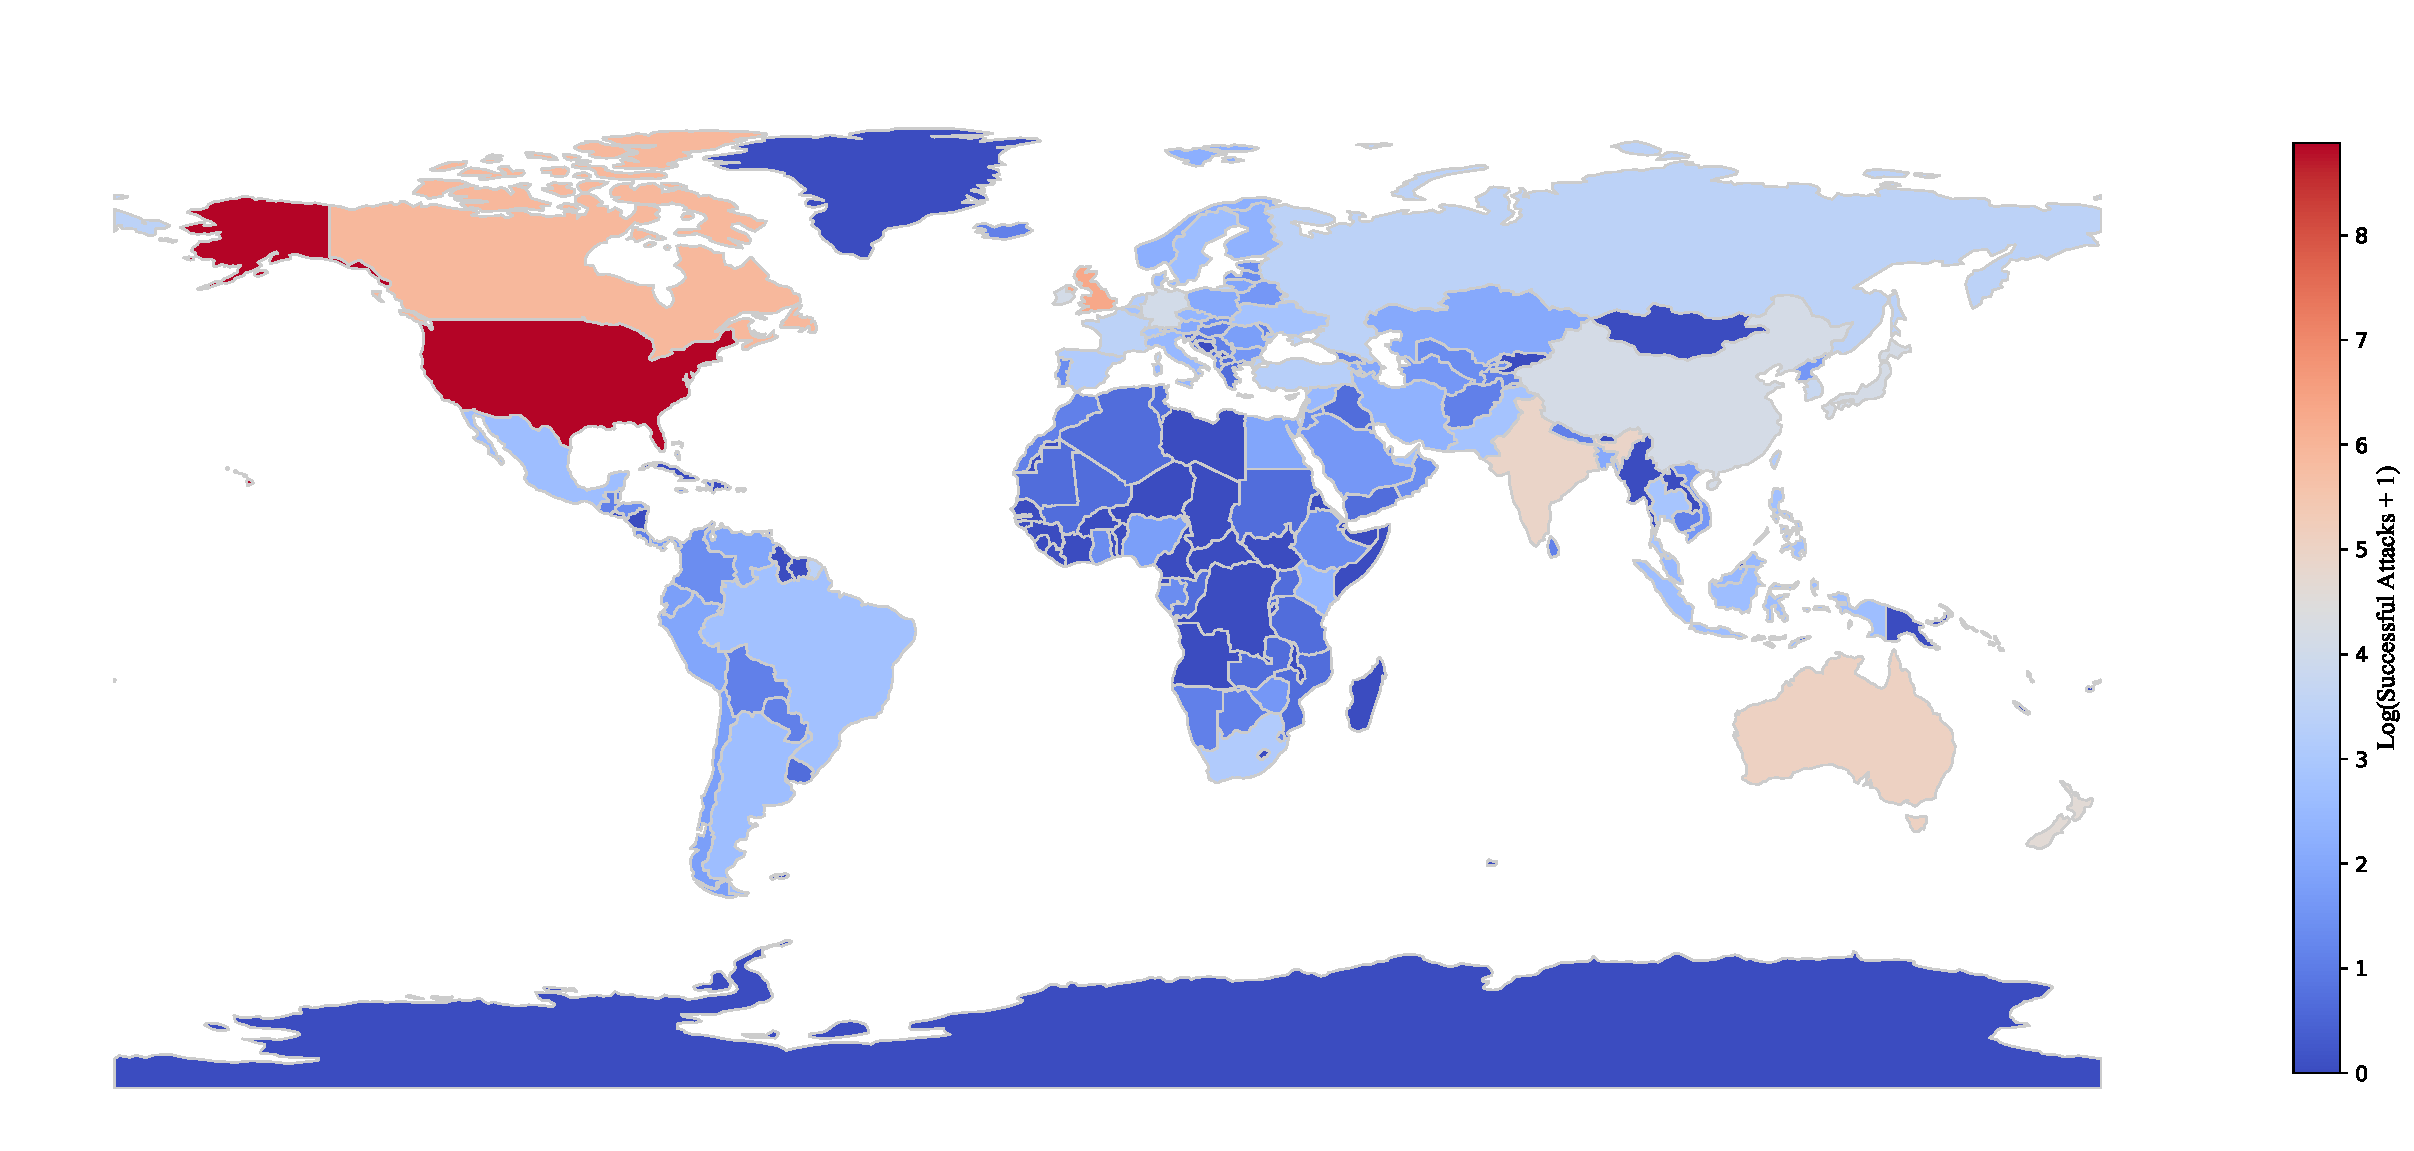
\includegraphics[width=0.8\linewidth]{../rsrc/distributions/Crime_Successful_distribution}
		}\\
		\subfloat[Mitigated Cybercrime Attempts]{
			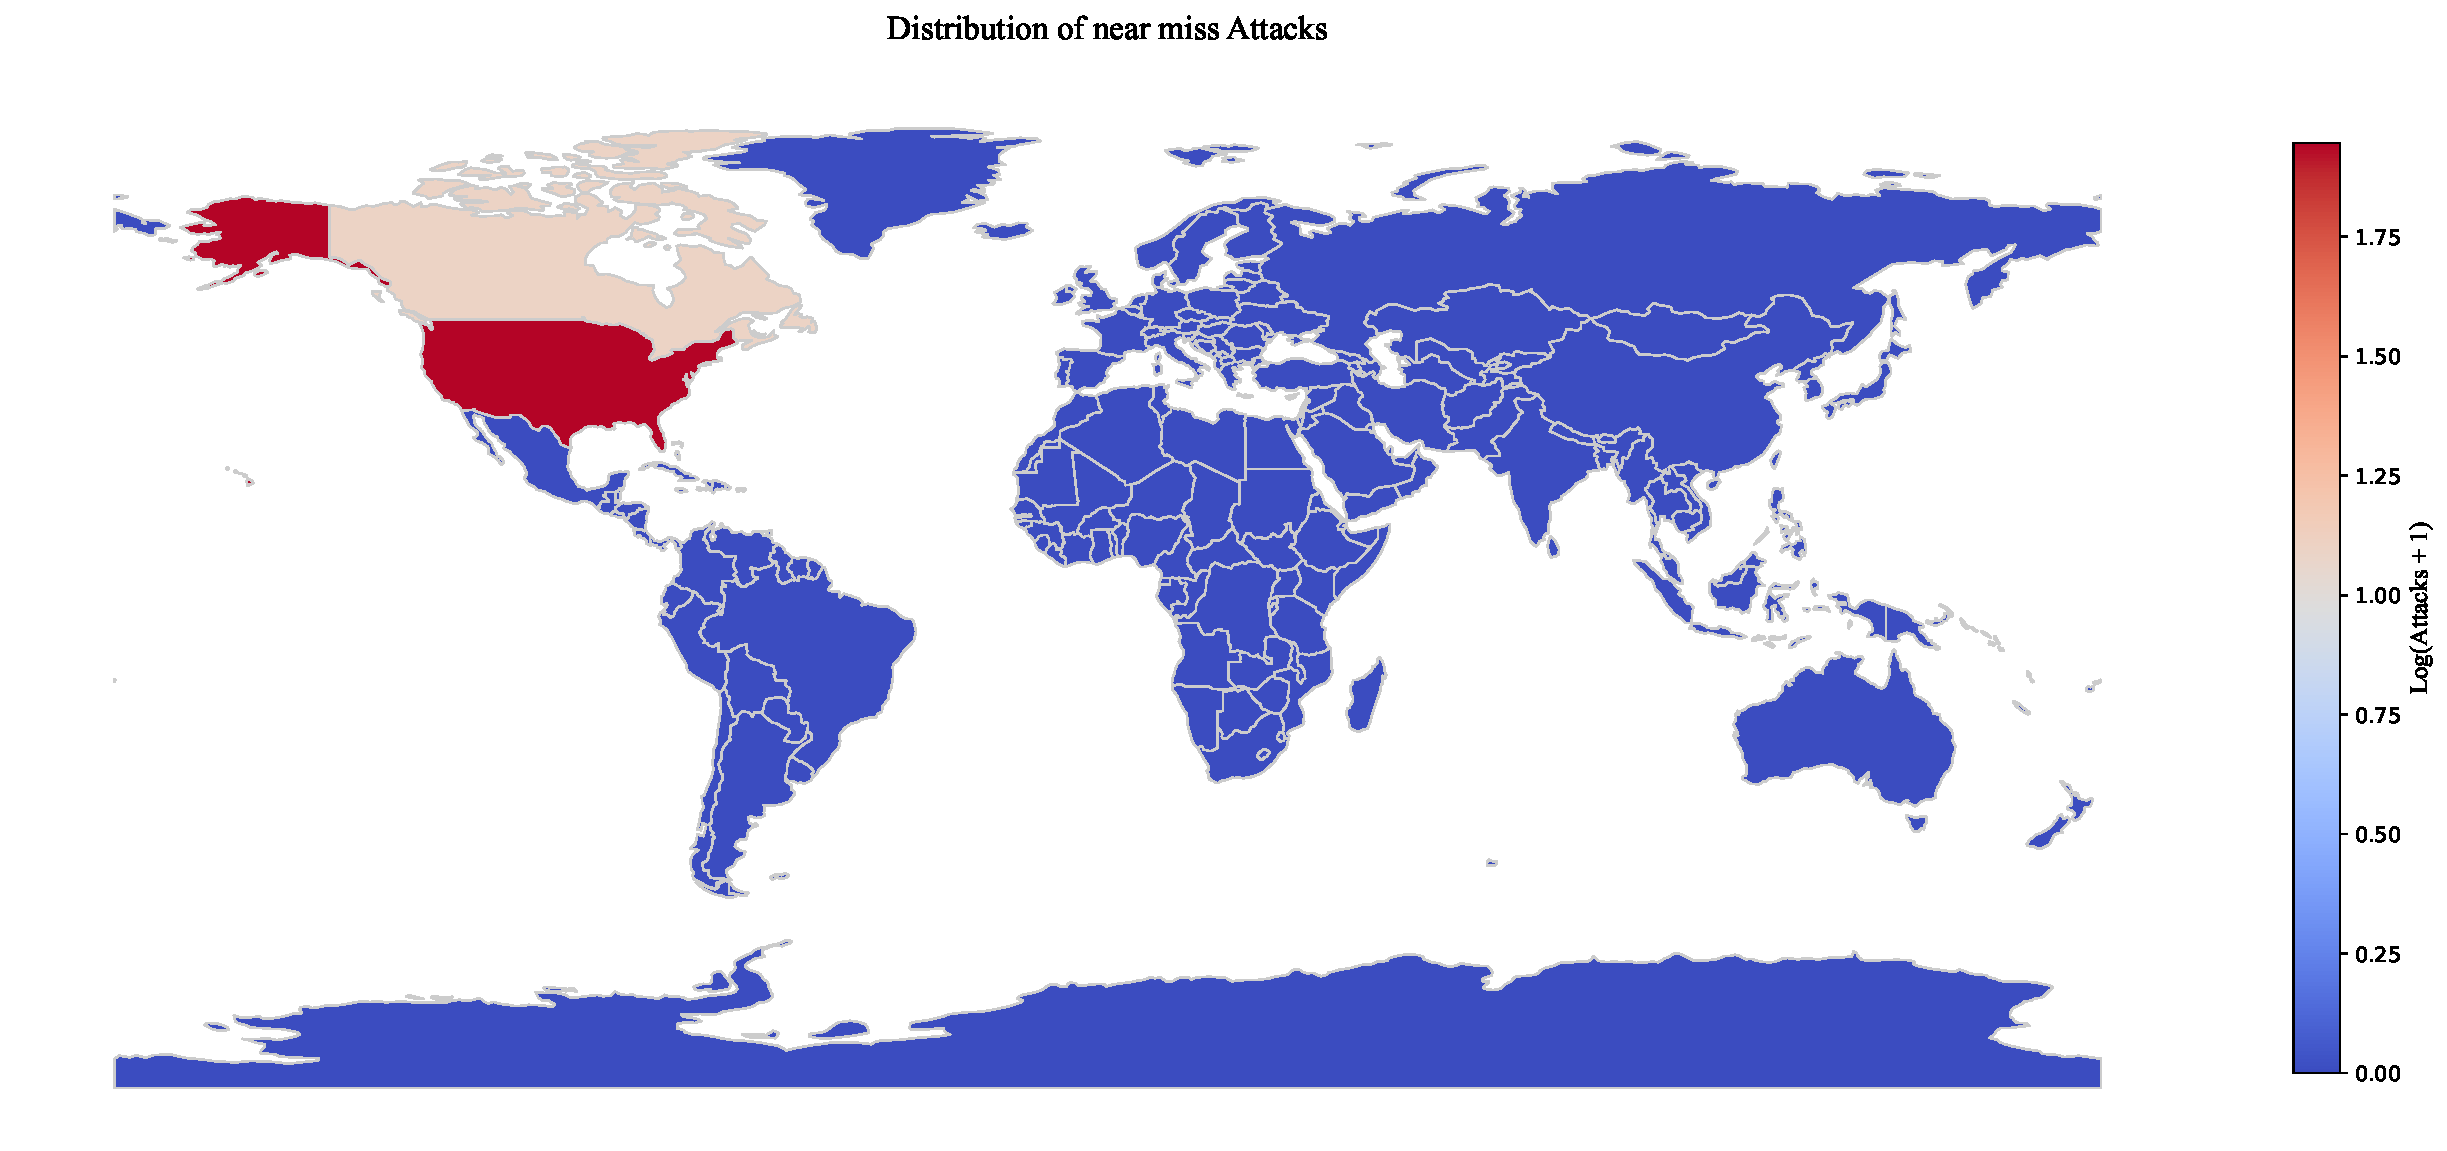
\includegraphics[width=0.4\linewidth]{../rsrc/distributions/Crime_NearMiss_distribution}
		}\hfill
		\subfloat[Reported Cybercrime Incidents]{
			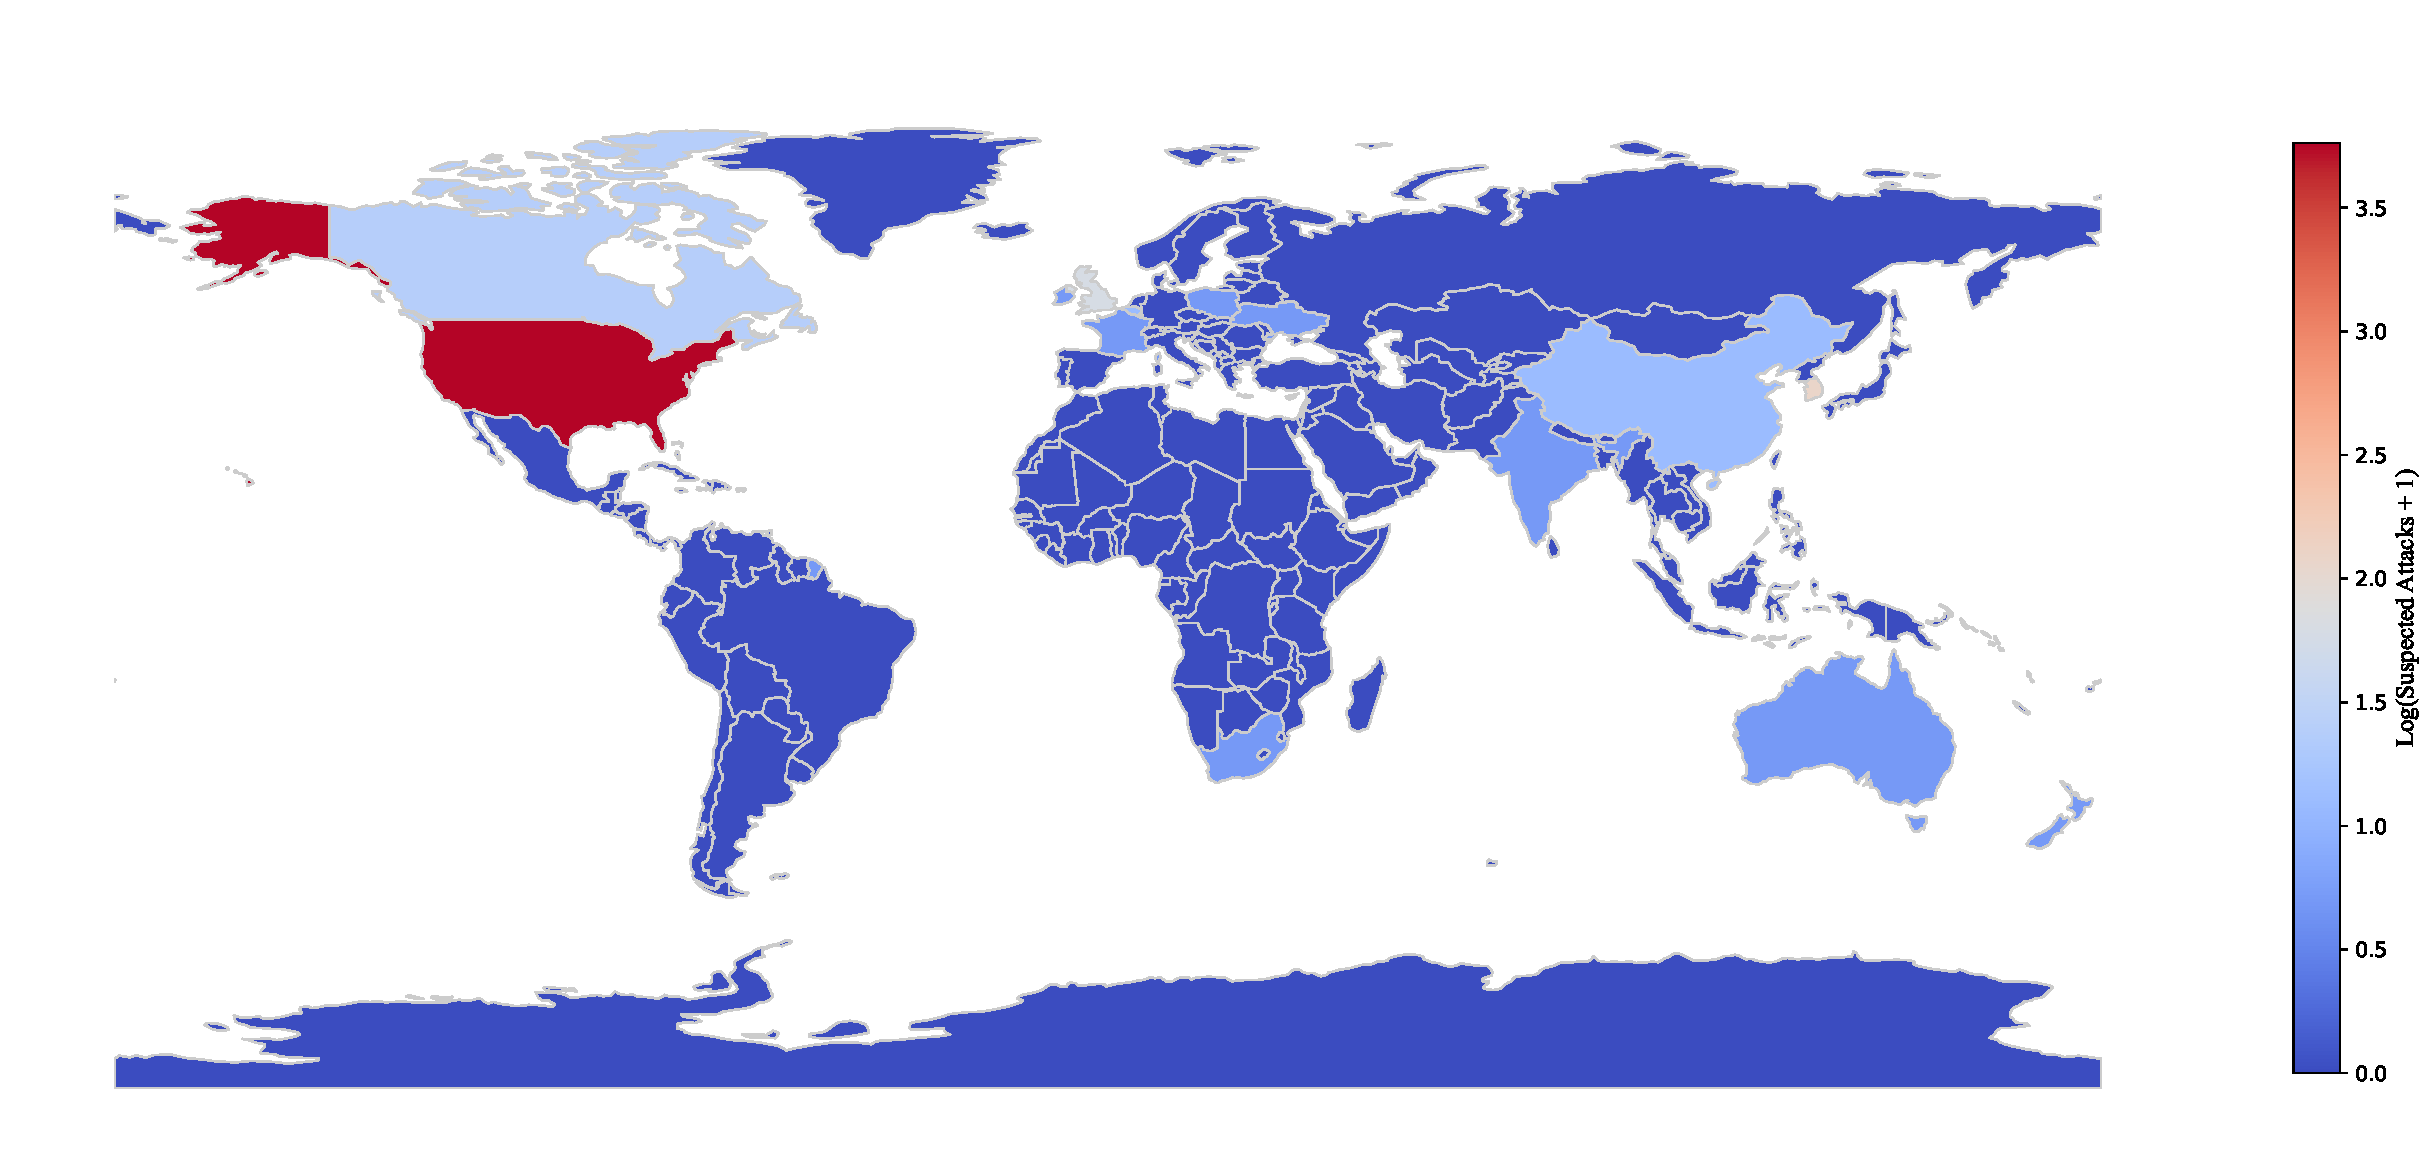
\includegraphics[width=0.4\linewidth]{../rsrc/distributions/Crime_Suspected_distribution}
		}\\
		\caption{Other Cybercrime Incidents}\label{fig:other-cybercrime-incidents}
	\end{figure}
\subsection{Pattern Discovery}\label{subsec:pattern-discovery} %3.4
	As illustrated in Figure~\ref{fig:other-cybercrime-incidents},
	the majority of countries worldwide lack adequate defensive capabilities against cyberattacks.
	Among the disclosed incidents, only the United States and Canada have recorded successful defense cases,
	with the United States reporting 6 instances and Canada reporting 2.
	This disparity can be attributed to the early development and technological maturity of the United States' cybersecurity infrastructure.
	The advanced technologies employed by both the U.S.\ government and private enterprises have enabled a certain level of resilience against some cyberattacks.
	Additionally, the disproportionately high volume of cybercrime in the United States plays a significant role.
	The extensive record of cyber incidents increases the likelihood of successful defenses,
	as it provides more opportunities for defensive mechanisms to be tested and refined.
	In contrast, other countries lack both the advanced defensive technologies and the high volume of cybercrime records that the United States possesses.
	Consequently, no successful defense cases have been reported for these countries in the VCDB .

	Cybercrime exhibits distinct patterns both across countries categorized by the GCI (Global Cybersecurity Index) and over time.
	To analyze these trends, we calculated the proportion of cybercrime incidents and visualized the results in Figure 2.
	This figure illustrates the annual average $hmD/P_i$ for each GCI tier (T1 to T5) from 2000 to 2025,
	providing a comprehensive overview of the spatial and temporal distribution of cybercrime.
	\begin{itemize}
		\item \textbf{2012 to 2016} Around 2012, both T5 and T1 countries exhibited the highest number of cybercrime incidents.
			Specifically, the $hmD/P_i$ index for T5 countries reached 86.63,
			marking the highest average number of cybercrime incidents among all tiers over the 25-year period.
			In contrast, T2, T3, and T4 countries reported significantly fewer incidents compared to T1 and T5 during this timeframe.
			The high cybercrime rates in T5 countries can be attributed to their poor performance across all five GCI assessment metrics:
			Legal, Technical, Organizational, Capacity Development, and Cooperation.
			These deficiencies likely contributed to their low GCI rankings and inadequate cybersecurity infrastructure,
			which in turn made them more vulnerable to cybercrime.
			On the other hand, T1 countries, despite their high GCI rankings, experienced a surge in cybercrime incidents around 2012.
			This suggests that even these nations were not fully prepared for the rapid evolution of cyber threats during this period.
			It is important to note that the fifth edition of the GCI assessment data was only released in 2024,
			meaning that the high rankings of T1 countries in 2024 do not necessarily reflect their cybersecurity capabilities in 2012.
		\item \textbf{2016 to 2020} During the period from 2016 to 2020, the number of cybercrime incidents declined across all tiers, from T1 to T5.
			Notably, T1 countries experienced a sharp decrease in cybercrime rates.
			This trend can be attributed to several factors.
			First, T1 countries, with their advanced technological infrastructure and robust cybersecurity policies,
			were better equipped to adapt to emerging threats.
			During this period, many T1 nations implemented comprehensive cybersecurity strategies,
			including stricter regulations, enhanced public-private partnerships, and increased investment in cybersecurity education and training.
			Additionally, international cooperation played a significant role in mitigating cross-border cyber threats.
			For example, initiatives such as information sharing through organizations like VERIS
			contributed to a more coordinated global response to cybercrime.
			However, despite the overall decline, T5 countries remained the most affected by cybercrime,
			likely due to their low performance in the GCI assessment metrics.
			These deficiencies continued to hinder their ability to build effective cybersecurity defenses,
			leaving them more vulnerable to cyber threats.
		\item \textbf{2020 till Present} Around 2020, a remarkable shift has occurred in the distribution of cybercrime incidents across the GCI tiers.
			Notably, the number of reported cybercrime incidents in T5 countries has dropped to almost negligible levels,
			a phenomenon that warrants further investigation.
			Similarly, T4 countries have maintained cybercrime rates comparable to those of T5.
			In contrast, T1, T2, and T3 countries continue to report a portion of cybercrime incidents,
			although these numbers have been steadily decreasing year by year.
			This trend may reflect the cumulative impact of sustained investments in cybersecurity infrastructure, policy improvements, and international collaboration among higher-tier countries.
			However, the sharp decline in T5 countries' cybercrime records remains puzzling and could be attributed to underreporting.
			Further research is needed to explore these potential explanations.
	\end{itemize}
 %3

\section{Policy Identification and Analysis}\label{sec:policy-identification-and-analysis}
To identify the effectiveness of national cybersecurity policies,
it is essential to analyze the correlation between the implementation of these policies and the subsequent trends in cybercrime.
By examining the distribution of cybercrimes and comparing it with the timing and content of various national policies,
we can discern patterns that highlight which measures are particularly effective or ineffective.
This analysis will focus on key metrics such as the reduction in
cybercrime incidents, the success rate of prosecutions, and the overall resilience of national cybersecurity infrastructures.
Through this data-driven approach,
we aim to provide actionable insights for the development and refinement of cybersecurity policies.
\subsection{Selection of Representative Centroid Countries}\label{subsec:selection-of-representative centroid-countries} %4.1
Having constructed a clustering model to categorize countries into five clusters (T1 to T5) based on GCI and other relevant metrics,
we now proceed to analyze the effectiveness of cybersecurity policies within each cluster.
To ensure a representative and data-driven analysis,
we will select one central country from each cluster that meets the following criteria:
\begin{itemize}
    \item \textbf{Representativeness:}
    The selected country should typify the overall characteristics of its cluster,
    reflecting the general trends and patterns observed within that group.
    \item \textbf{Data Availability:}
    The country must have sufficient historical data on cybersecurity policies and legislation enacted over the past two decades,
    allowing for a comprehensive analysis of policy impacts.
\end{itemize}
By focusing on these representative countries,
we aim to draw meaningful insights into the effectiveness of various cybersecurity policies and laws,
which can then be generalized to other countries within the same cluster.

To identify the representative country for each cluster,
we first calculate the average Global Cybersecurity Index (GCI) for each cluster.
The average GCI, denoted as \(\overline{GCI}\), is computed as follows:
\[ \overline{GCI} = \frac{\sum_{i=1}^{n} GCI_i}{n} \]
where \(n\) is the number of countries in the cluster.
Next, we compute the absolute deviation of each country's GCI from the cluster average:
\[|GCI_i - \overline{GCI}|\] .
The country with the smallest deviation is considered the most representative of its cluster.
After this initial selection, we further filter out countries with insufficient or incomplete legal and policy documentation.

Through this process, we identify the following representative countries for each cluster:
\begin{itemize}
    \item \textbf{T1: United States}
    ~\cite{
        congress-website,
        nist-website,
        dhs-website,
        sec-website,
        whitehouse-website,
        investigatory-powers-act-2016,
        ncsc-uk,
        telecom-security-act-2021,
        uk-cyber-security-requirements-2024,
        uk-cybersecurity-timeline-2024}
    \item \textbf{T2: Japan}
    ~\cite{
        it-basic-law-japan,
        ppc-legal-japan,
        nisc-japan,
        mofa-japan,
        japan-law-translation,
        cs-strategy-2015-japan,
        cs-strategy-2018-japan,
        telecom-business-act-japan,
        cs-strategy-2021-japan}
    \item \textbf{T3: China}
    ~\cite{
        international-cybercrime,
        cybersecurity-law-china,
        internet-censorship-china,
        china-data-security-regulations,
        cryptography-law-china}
    \item \textbf{T4: Costa Rica}
    ~\cite{
        costa-rica-cybersecurity-strategy,
        costa-rica-pop-up}
    \item \textbf{T5: Namibia}
    ~\cite{
        namibia-pop-up,
        namibia-digital-odyssey,
        namibia-cybersecurity-strategy}
\end{itemize}
 %4

\section{Correlation Between National Demographics and Cybercrime Distribution}
\label{sec:correlation-between-national-demographics-and-cybercrime-distribution}
%! Author = Yilin
%! Date = 2025/1/27

The distribution of cybercrime is closely tied to national demographic statistics,
with the number of cybercrime incidents showing a positive correlation with several key factors.
In this section, we explore the relationship between cybercrime and four primary demographic indicators:
the proportion of internet users in a country,
the country's GDP, and the proportion of the population with higher education.
By analyzing these factors,
we aim to uncover patterns and correlations that can provide insights into the drivers of cybercrime
and inform the development of more targeted and effective cybersecurity policies.
\subsection{Data Preprocessing}\label{subsec:data-preprocessing} %5.1
    To analyze the correlation between national demographics and cybercrime distribution,
    we first preprocess the relevant data.
    The demographic indicators—internet user penetration\cite{it-net-user-zs}, 
    GDP\cite{ny-gdp-mktp-cd} and 
    the proportion of the population with higher education\cite{se-ter-enrr}
    —are obtained from the World Bank's official website.
    Additionally, we utilize the annual cybercrime incident data for each country,
    which was previously processed in our earlier analysis.
    By integrating these datasets,
    we ensure a comprehensive foundation for examining the relationship between demographic factors and cybercrime trends.
    \begin{itemize}[label=\phantom{.}, leftmargin=-0.18em]
        \item \textbf{Data Integration and Cleaning}: \\
            For each dataset, we filter the data to include only the years from 2010 to 2022.
            After filtering,
            we handle missing values by allowing a maximum missing value proportion of 20\% for each country's data.
            Missing values within this threshold are filled using linear interpolation.
            Any data points that remain missing after interpolation
            are removed to ensure the integrity and reliability of the dataset.
            This preprocessing step ensures that our analysis is based on a consistent and high-quality dataset.
    \end{itemize}


\subsection{Data Processing and Analysis}\label{subsec:data-processing-and-analysis} %5.2
    \subsubsection{Data Consolidation} %5.2.1
        After preprocessing the individual datasets, we integrate the internet user data and the cybercrime incident data.
        This is achieved by performing an inner join on the two datasets using country codes and years as the matching keys.
        The inner join ensures that only the countries and years present in both datasets are retained,
        resulting in a combined dataset where each entry corresponds to a specific country and year with complete data
        for both internet user penetration and cybercrime incidents.
        This step is crucial for ensuring the accuracy and consistency of our subsequent analysis.

    \subsubsection{Logarithmic Transformation} %5.2.2
        To address the skewness in the distribution of cybercrime incident counts,
        we apply a logarithmic transformation to the data.
        As described in Subsection~\ref{subsec:building-the-hotspot-map},
        we use the \textit{log1p} transformation, which computes the natural logarithm of \(1 + x\),
        where \(x\) is the original cybercrime count.
        This transformation reduces the impact of extreme values and makes the data more symmetric,
        bringing it closer to a normal distribution.
        By applying this transformation, we ensure that the data is better suited for statistical analysis and modeling.

    \subsubsection{Spearman Correlation Analysis} %5.2.3
        To quantify the relationship between those data and the number of cybercrime incidents,
        we calculate the Spearman correlation coefficient.
        This non-parametric measure assesses the strength and direction of the monotonic relationship between two variables.
        The Spearman correlation coefficient (\(\rho\)) and its associated \(p\)-value are computed,
        with the \(p\)-value used to determine the statistical significance of the correlation.
        A \(p\)-value smaller than \(1 \times 10^{-10}\) indicates an extremely strong statistical significance.
        The Spearman correlation coefficient is calculated as follows:
        \[ \rho = 1 - \frac{6 \sum d_i^2}{n(n^2 - 1)} \]
        where:
        \begin{itemize}
            \item \(\rho\) is the Spearman rank correlation coefficient,
            \item \(d_i\) is the difference between the ranks of each pair of observations, and
            \item \(n\) is the number of observations.
        \end{itemize}

\subsection{Data Visualization}\label{subsec:data-visualization} %5.3
To further explore the relationship between demographic factors and cybercrime,
we generate several visualizations.
These include scatter plots, time series plots, and distribution plots,
all of which are presented on a logarithmic scale
due to the logarithmic transformation applied during data preprocessing.

    \subsubsection{Scatter Plots} %5.3.1
        We begin by plotting scatter diagrams to visualize the relationship between demographic indicators
        (such as internet user penetration, higher education enrollment, and GDP) and the logarithmically transformed cybercrime counts.
        A regression line is added to each scatter plot to highlight the trend.
        The Spearman correlation coefficient (\(\rho\)) and its associated \(p\)-value are annotated on the plots to provide statistical context.
        For example:
        \begin{itemize}
            \item The scatter plot for \textbf{internet user penetration}
                shows a correlation coefficient of \(\rho = 0.17\) with a highly significant \(p\)-value of \(2.33 \times 10^{-12}\).
            \item The scatter plot for \textbf{higher education enrollment}
                reveals a correlation coefficient of \(\rho = 0.13\) with a \(p\)-value of \(2.60 \times 10^{-5}\).
            \item The scatter plot for \textbf{GDP}
                indicates a weaker correlation (\(\rho = 0.45\)) but with an extremely low \(p\)-value of \(2.456 \times 10^{-87}\),
                suggesting a statistically significant relationship.
        \end{itemize}

    \subsubsection{Time Series Plots} %5.3.2
        Next, we construct time series plots to analyze the temporal trends in cybercrime and GDP .
        These plots display the annual average of logarithmically transformed cybercrime counts and GDP over time,
        allowing us to observe how these variables have evolved from 2010 to 2022.
        The time series plot for GDP reveals a steady increase over the years,
        while cybercrime counts show fluctuations with a general upward trend.
        Figure~\ref{fig:gdp}.
        \begin{figure}[htbp]
            \centering
            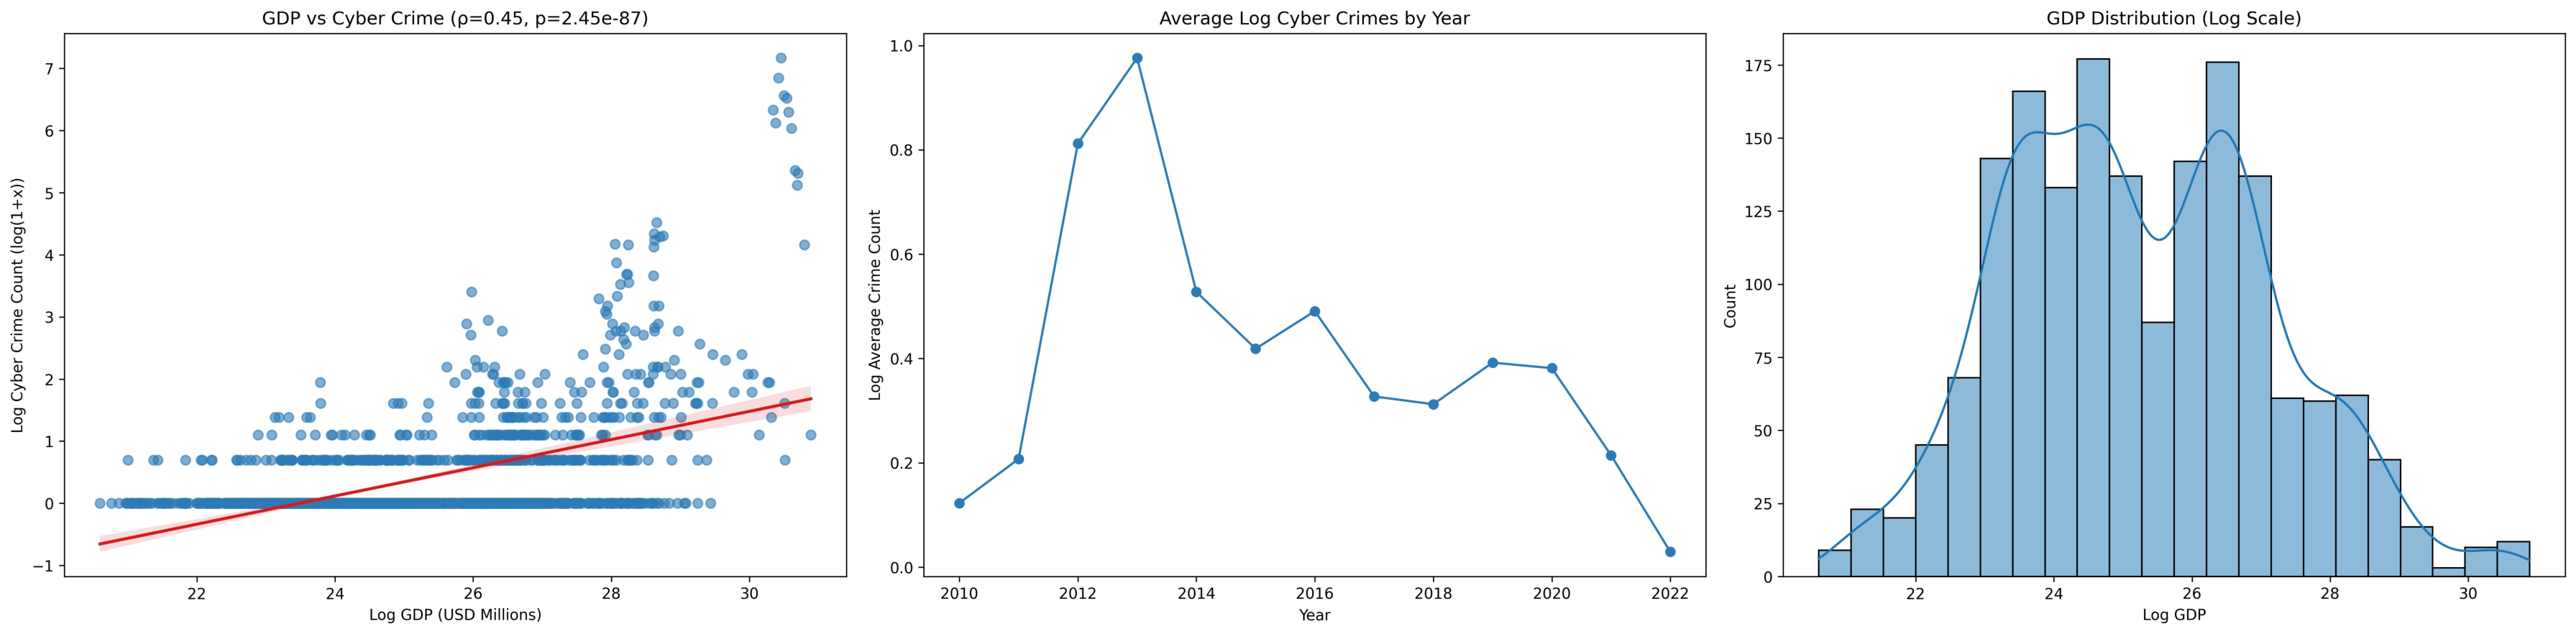
\includegraphics[width=1\linewidth]{../rsrc/demographics/gdp_crime_and_time}
            \caption{GDP Chart}\label{fig:gdp}
        \end{figure}

    \subsubsection{Distribution Plots} %5.3.3
        Finally, we generate distribution plots to examine the spread and density of the data.
        These plots illustrate the distribution of demographic indicators
        (e.g., internet user penetration, higher education enrollment) and their relationship with cybercrime counts.
        For example:
        \begin{itemize}
            \item The distribution plot for \textbf{internet user penetration} shows a right-skewed distribution,
                indicating that most countries have relatively low internet penetration rates.
                Figure~\ref{fig:internet}.
            \item The distribution plot for \textbf{higher education enrollment} reveals a more uniform distribution,
                with a peak around 60--80\% enrollment rates.
                Figure~\ref{fig:education}.
        \end{itemize}
        \begin{figure}[htbp]
            \centering
            \subfloat{
                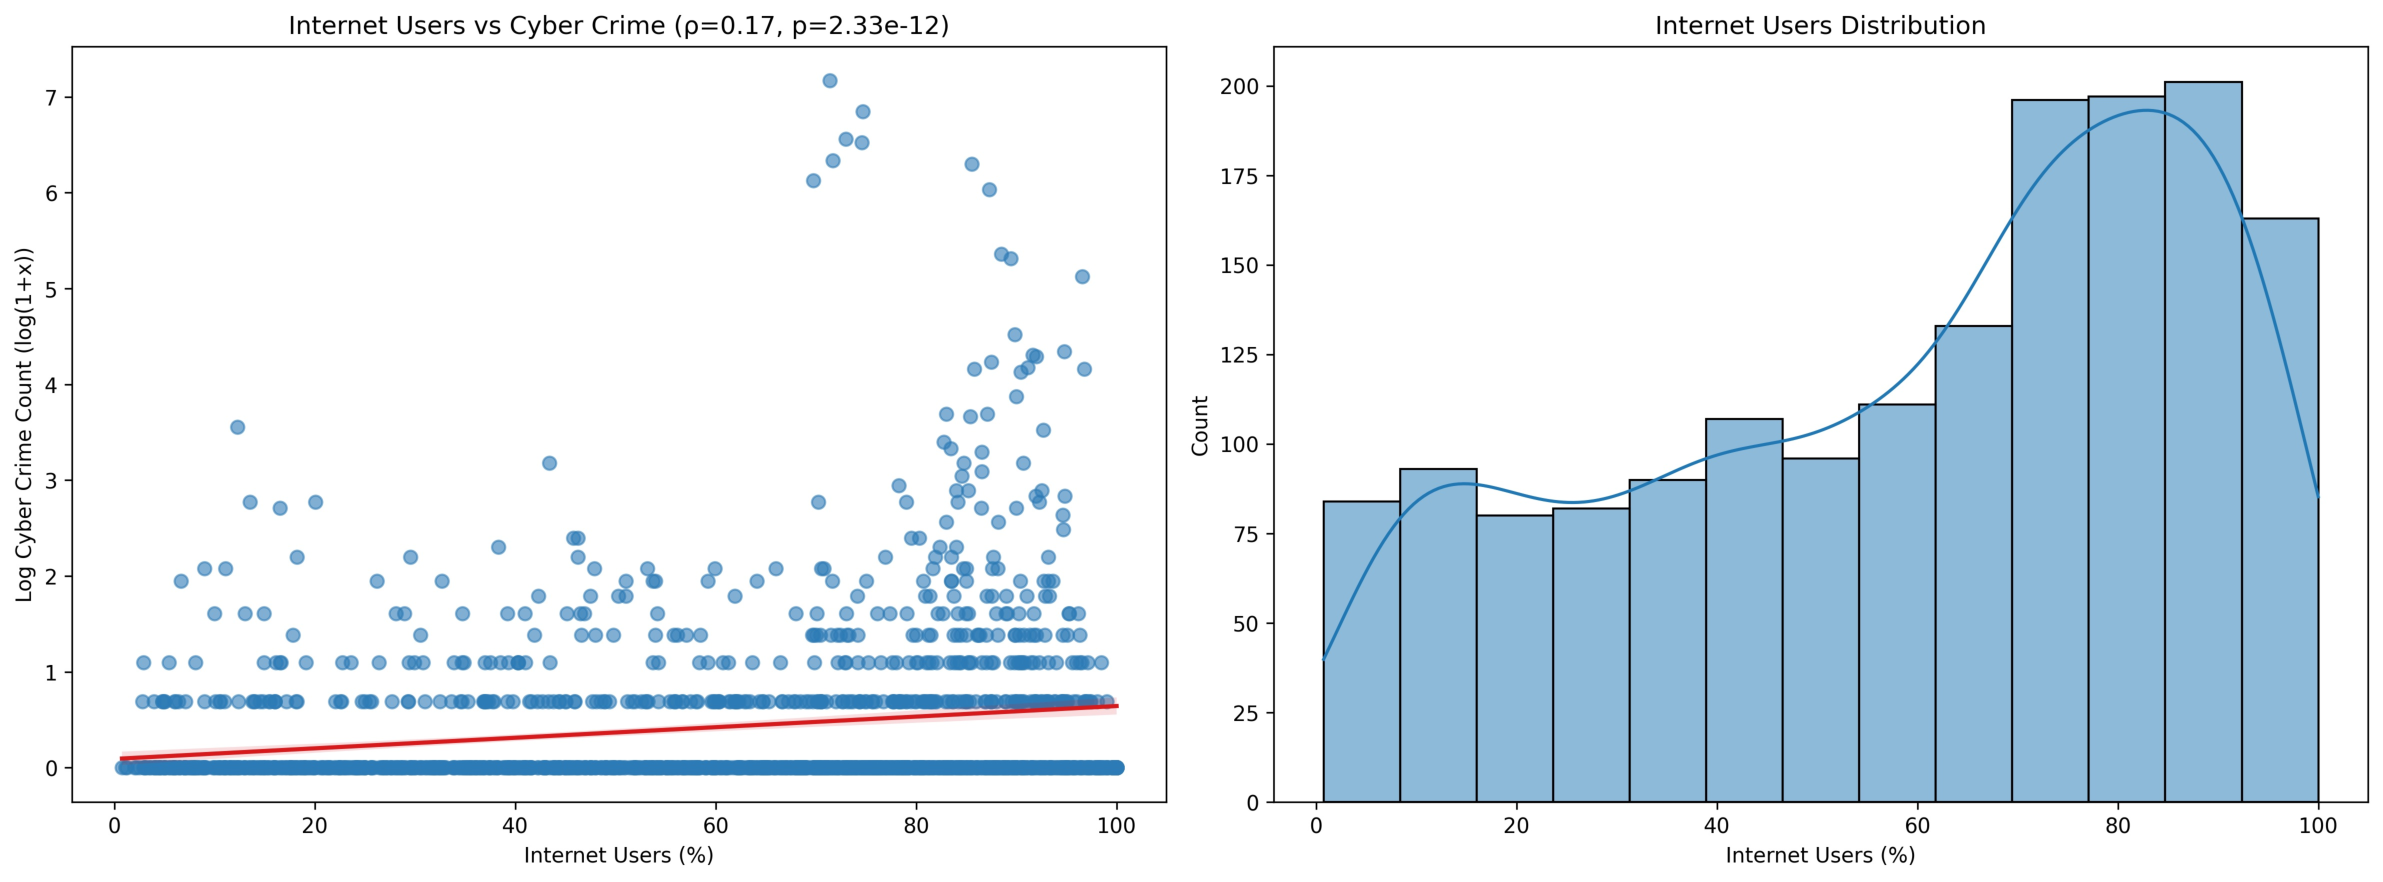
\includegraphics[width=0.8\linewidth]{../rsrc/demographics/Internet Users}\label{fig:internet}
            }\\
            \subfloat{
                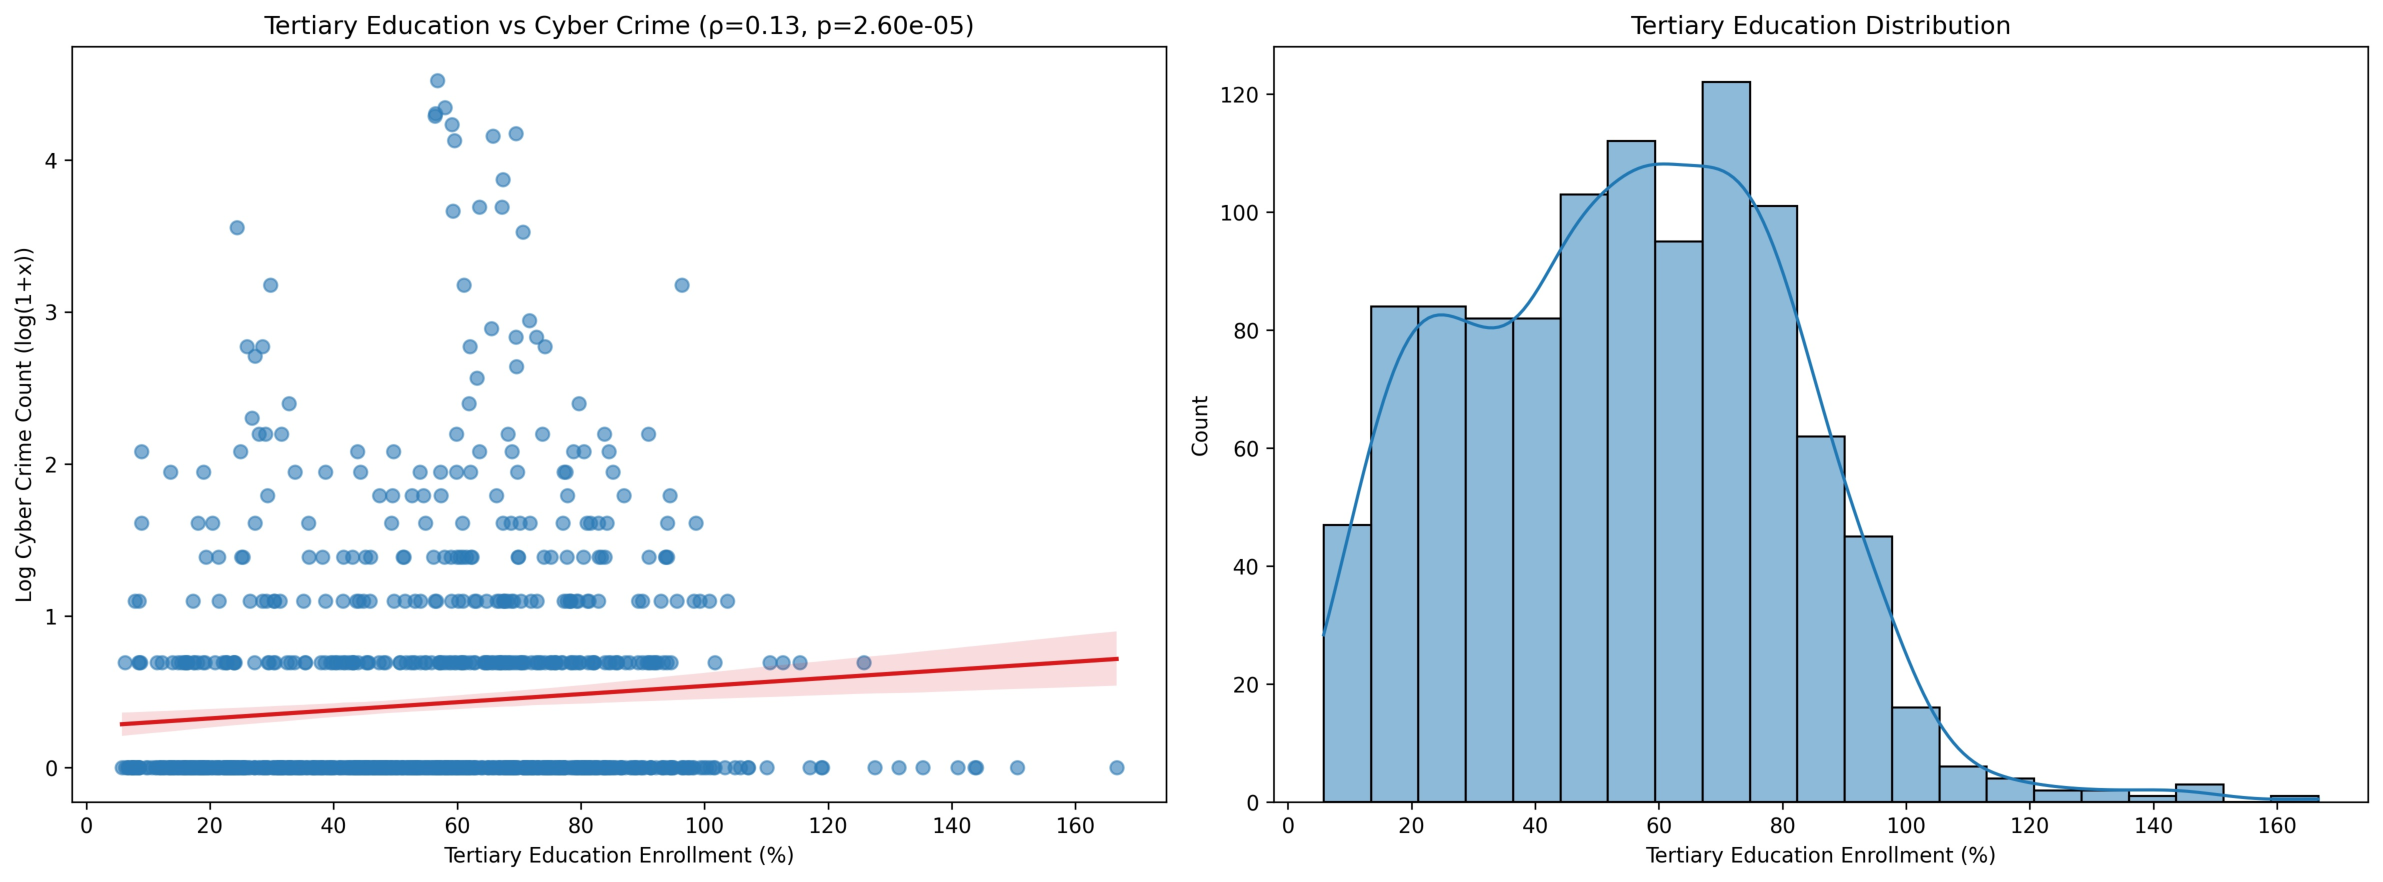
\includegraphics[width=0.8\linewidth]{../rsrc/demographics/Tertiary Education}\label{fig:education}
            }\\
            \caption{Trends and Correlations Related to Cybercrime}
        \end{figure}

    \subsubsection{Model Comparison: TOPSIS} %5.3.4
        \begin{enumerate}
            \item \textbf{Data Standardization}
                Standardize raw data to eliminate dimensional differences.
                For each indicator \(j\):
                - \textbf{Positive indicators} (higher values are better):
                \[
                    x_{ij}^* = \frac{x_{ij} - \min(x_j)}{\max(x_j) - \min(x_j)}
                \]
                - \textbf{Negative indicators} (lower values are better):
                \[
                    x_{ij}^* = \frac{\max(x_j) - x_{ij}}{\max(x_j) - \min(x_j)}
                \]
                where \(x_{ij}\) is the raw value of the \(i\)-th country for the \(j\)-th indicator.
            \item \textbf{Entropy-Based Weight Calculation} \\
                1. Calculate the probability distribution of standardized values:
                \[
                    p_{ij} = \frac{x_{ij}^*}{\sum_{i=1}^n x_{ij}^*}, \quad e_j = -\frac{1}{\ln n} \sum_{i=1}^n p_{ij} \ln p_{ij} \quad (p_{ij} \ln p_{ij} = 0 \text{ if } p_{ij}=0).
                \]
                2. Derive weights from entropy values:
                \[
                    w_j = \frac{1 - e_j}{\sum_{k=1}^m (1 - e_k)}.
                \]
            \item \textbf{Weighted Standardized Matrix}
                Construct the matrix \(V\) by combining standardized data with weights:
                \[
                    v_{ij} = w_j \cdot x_{ij}^*, \quad V = [v_{ij}]_{n \times m}.
                \]
            \item \textbf{Ideal Solutions}
                Define the ideal (\(S^+\)) and negative-ideal (\(S^-\)) solutions:
                \[
                    S^+ = \left\{ \max_{i}(v_{ij}) \mid j=1,2,\dots,m \right\}, \quad S^- = \left\{ \min_{i}(v_{ij}) \mid j=1,2,\dots,m \right\}.
                \]
            \item \textbf{Ranking via Relative Closeness} \\
                1. Calculate Euclidean distances to ideal solutions:
                \[
                    D_i^+ = \sqrt{\sum_{j=1}^m (v_{ij} - S_j^+)^2}, \quad D_i^- = \sqrt{\sum_{j=1}^m (v_{ij} - S_j^-)^2}.
                \]
                2. Compute relative closeness for ranking:
                \[
                    C_i = \frac{D_i^-}{D_i^+ + D_i^-}, \quad \text{where } C_i \in [0,1]. \quad (C_i \to 1 \text{ indicates better performance}).
                \]
        \end{enumerate}

        The Pearson correlation matrix (see Appendix~\ref{fig:correlation-matrix}) reveals critical insights into the relationships between key variables.
        Notably, \textbf{crime rates} exhibit a significant negative correlation with \textbf{education levels} (\(r = -0.13^*\)),
        suggesting that regions with higher educational attainment may experience reduced criminal activity, consistent with human capital theory.
        Similarly, \textbf{law enforcement intensity} (Warrant) shows a moderate negative association with crime rates (\(r = -0.25\)),
        reinforcing the deterrent effect of robust policing.
        The strongest observed correlation involves \textbf{risk prevention measures} (Risk),
        which display a pronounced negative relationship with crime rates (\(r = -0.50\) to \(-0.75\)),
        implying that targeted risk mitigation strategies could substantially curb criminal behavior.

        Among socioeconomic factors, \textbf{GDP} is positively correlated with \textbf{data reporting completeness} (\(r = 0.17^{**}\)),
        indicating that economically developed regions tend to have more reliable crime monitoring systems.
        Conversely, \textbf{internet penetration} demonstrates only a weak, non-significant link to crime rates (\(r = 0.1\)),
        highlighting its limited direct influence in the current model.

        \noindent \textit{Note: \(^*p < 0.05\), \(^{**}p < 0.01\). Variable definitions are provided in Appendix A.}

        \begin{figure}
            \centering
            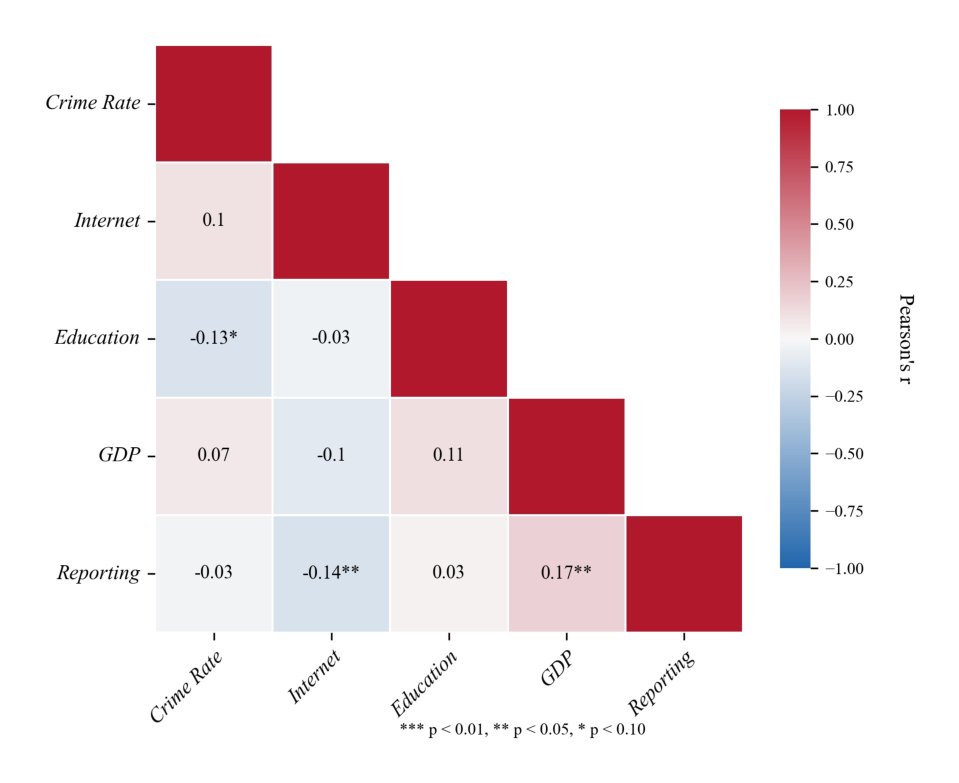
\includegraphics[width=0.75\linewidth]{../rsrc/demographics/correlation_matrix}
            \caption{Correlation Matrix}\label{fig:correlation-matrix}
        \end{figure}
 %5

\section{Future Work}\label{sec:future-work} %6
%! Author = Mei
%! Date = 2025/1/27

To enhance the model's robustness and applicability, several improvements are proposed.
\begin{itemize}
    \item Incorporating \textbf{time-series} or \textbf{panel data analysis} would capture dynamic effects,
        such as the lagged impacts of policy changes on crime rates.
    \item Integrating \textbf{machine learning} methods like random forests
        could better handle nonlinear relationships and complex variable interactions,
        addressing limitations of linear models.
    \item Developing a simplified \textbf{visualization tool} to translate complex model results
        into easily interpretable charts would improve accessibility for policymakers,
        facilitating more informed decision-making.
\end{itemize}
These steps aim to address current limitations and expand the model's practical utility.


\section{Strength \& Weakness}\label{sec:strength-&-weakness}
%! Author = Yilin
%! Date = 2025/1/27

\subsection{As for the 1^{st} Question} %7.1
    By filtering the data and drawing the global heat map of cybercrime distribution,
    the global distribution of cybercrime can be visualized.
    Then, by filtering the data according to specific indicators
    (Confirmed, Near miss, Reported, Prosecuted)
    and drawing the corresponding global heat map,
    the distribution of these indicators can be visualized.

    Pure data screening and analysis need to be based on a huge amount of data.
    For these big countries in Europe and the United States, the annual amount of data is very considerable,
    so the effect is very prominent.
    But for some small countries in Africa or Asia,
    the difference in the distribution map of cybercrime is not very obvious because of the insufficient amount of data.

\subsection{As for the 2^{nd} Question} %7.2
    \begin{enumerate}
        \item Through processing the filtered data and drawing a line chart,
            it can be more intuitive to see which laws and policies have benefits for the national cybercrime rate control;
            However, the timeliness of legal policies cannot be rationally judged, that is,
            whether the law has an impact on the future cannot be directly considered.
        \item Introduction of Poisson model: Because the number of cybercrimes is a typical non-negative integer data,
            Poisson regression analysis can avoid the continuity assumption of ordinary linear regression,
            and can model and explain the nonlinear association between the number of bills and the crime rate and zero inflation data.
            Furthermore, the regression coefficients can be used for policy evaluation by calculating the incidence ratio $IRR$ .
            Over-discretization of the data can lead to bias in the model,
            and the model will only work for relationships that are roughly linear,
            and it will be less useful if the actual relationship is more complex (e.g., if there are interaction effects).
        \item Introduction of time hysteresis effect:
            The introduction of time lag effect can reflect the delay of the policy coming into effect, that is,
            the release of legal policies does not necessarily produce benefits at the time but will have potential impacts on the future.
            Then, the optimal lag period was selected by cross validation,
            and the key time node for the policy to be effective was clarified.
            But it ignores the immediate effect on the law.
    \end{enumerate}
    Therefore, it is necessary to combine the data analysis and Poisson \& time lag effect model
    to obtain the income effect of legal policies on the national Internet crime rate.

 %7

\bibliographystyle{unsrt}
\bibliography{references} %8

%\section*{Appendix}\label{sec:appendix} %9

\newpage
\section*{\centerline{\underline{Report on Use of AI}}}
\begin{enumerate}
	% 1. United States
    \item \textbf{OpenAI ChatGPT( Jan 25, 2025 version, ChatGPT-4o(Internet Search) )}
    \begin{description}
        \item Query1: Please give me more US cybersecurity laws and regulations from 2000 to 2023.
        \item Output: Here is a list of significant U.S.\ cybersecurity laws and regulations from 2000 to 2023:
        \begin{enumerate}[label=\arabic*.]
        		\item USA PATRIOT Act (2001)
			\begin{itemize}
				\item Expanded law enforcement’s ability to surveil and intercept communications for counterterrorism purposes, including provisions affecting cybersecurity.
			\end{itemize}
			\item Federal Information Security Management Act (FISMA) (2002)
			\begin{itemize}
				\item Required federal agencies to develop, document, and implement programs to secure information and systems.
			\end{itemize}
			\item Cybersecurity Research and Development Act (2002)
			\begin{itemize}
				\item Funded research and development for cybersecurity tools and technologies through the National Science Foundation (NSF) and National Institute of Standards and Technology (NIST).
			\end{itemize}
			\item E-Government Act (2002)
			\begin{itemize}
				\item Established guidelines for improving electronic government services, including the management of information security.
			\end{itemize}
			\item Homeland Security Act (2002)
			\begin{itemize}
				\item Created the Department of Homeland Security (DHS) and included provisions for critical infrastructure protection against cyber threats.
			\end{itemize}
			\item Presidential Policy Directive 21 (PPD-21) (2013)
			\begin{itemize}
				\item Aimed to strengthen critical infrastructure security and resilience, emphasizing information sharing across sectors.
			\end{itemize}
			\item National Institute of Standards and Technology (NIST) Cybersecurity Framework (2014)
			\begin{itemize}
				\item Voluntary guidelines for private and public organizations to manage and reduce cybersecurity risks.
			\end{itemize}
			\item Cybersecurity Information Sharing Act (CISA) (2015)
			\begin{itemize}
				\item Enabled the sharing of cyber threat information between private entities and the federal government.
			\end{itemize}
			\item Federal Cybersecurity Enhancement Act (2015)
			\begin{itemize}
				\item Mandated the use of intrusion detection and prevention systems (e.g., EINSTEIN) on federal networks.
			\end{itemize}
			\item National Defense Authorization Act (NDAA) Provisions (2019)
			\begin{itemize}
				\item Introduced supply chain security measures and banned federal agencies from using certain Chinese-made telecommunications equipment.
			\end{itemize}
			\item CLOUD Act (2018)
			\begin{itemize}
				\item Clarified legal processes for accessing electronic data stored abroad while balancing privacy and law enforcement interests.
			\end{itemize}
			\item SEC Guidelines on Cybersecurity Disclosure (2018, Updated 2023)
			\begin{itemize}
				\item Required public companies to disclose cybersecurity risks, incidents, and governance strategies to protect investors.
			\end{itemize}
			\item Internet of Things (IoT) Cybersecurity Improvement Act (2020)
			\begin{itemize}
				\item Set baseline security standards for IoT devices used by federal agencies.
			\end{itemize}
			\item Cyber Incident Reporting for Critical Infrastructure Act (CIRCIA) (2022)
			\begin{itemize}
				\item Required critical infrastructure operators to report significant cyber incidents within 72 hours and ransomware payments within 24 hours.
			\end{itemize}
			\item Quantum Computing Cybersecurity Preparedness Act (2022)
			\begin{itemize}
				\item Directed federal agencies to migrate to quantum-resistant cryptographic standards.
			\end{itemize}
			\item Strengthening American Cybersecurity Act (2022)
			\begin{itemize}
				\item Consolidated multiple cyber laws, introduced new rules for incident reporting, and enhanced federal cybersecurity protections.
			\end{itemize}
			\item CHIPS and Science Act (2022)
			\begin{itemize}
				\item Included cybersecurity measures for semiconductor manufacturing and technology development.
			\end{itemize}
			\item Telecommunications Supply Chain Security (2023)
			\begin{itemize}
				\item Expanded restrictions on telecommunications companies deemed national security risks.
			\end{itemize}
        \end{enumerate} \\
    \end{description}

	% 2. Japan
    \item \textbf{OpenAI ChatGPT( Jan 25, 2025 version, ChatGPT-4o(Internet Search) )}
    \begin{description}
		\item Query2: Also give me the laws and regulations related to network security in Japan from 2000 to the present.
		\item Output: Here are Japan’s key cybersecurity-related laws and policies from 2000 to the present,:
        \begin{enumerate}[label=\arabic*.]
        		\item Basic Act on the Formation of Advanced Information and Telecommunications Network Society (2000)
			\begin{itemize}
				\item Established a framework for building advanced information and telecommunications society in collaboration with public and private sectors.
			\end{itemize}
			\item Act on the Protection of Personal Information (2003)
			\begin{itemize}
				\item Japan’s first law focusing on personal information protection, setting rules for the collection, use, and management of personal data.
			\end{itemize}
			\item Comprehensive Strategy on Information Security (2003)
			\begin{itemize}
				\item Introduced by the Ministry of Economy, Trade, and Industry (METI), emphasizing the concept of a “society assuming accidents,” aiming to prevent and mitigate cybersecurity incidents.
			\end{itemize}
			\item Basic Plan on Information Security (2006)
			\begin{itemize}
				\item Proposed a “new public-private partnership model,” clarifying roles and cooperation between the government and private sector in ensuring information security.
			\end{itemize}
			\item Cybersecurity Strategy (2013)
			\begin{itemize}
				\item Japan’s first cybersecurity strategy, addressing comprehensive challenges in cyberspace and advocating for international collaboration.
			\end{itemize}
			\item Basic Act on Cybersecurity (2014)
			\begin{itemize}
				\item Passed in November 2014, it defined the responsibilities of governmental, private, and academic institutions in promoting cybersecurity and established the Cybersecurity Strategic Headquarters.
			\end{itemize}
			\item Cybersecurity Strategy (2015)
			\begin{itemize}
				\item Highlighted Japan’s vision of ensuring “a free, fair, and secure cyberspace” and aligned with international cybersecurity standards.
			\end{itemize}
			\item Cybersecurity Strategy (2018)
			\begin{itemize}
				\item Updated the 2015 strategy by including concrete action plans, enhancing organizational frameworks, and strengthening international cooperation.
			\end{itemize}
			\item Telecommunications Business Act Amendments (2019)
			\begin{itemize}
				\item Introduced measures to ensure the security of telecommunications infrastructure, including vendor restrictions for critical infrastructure.
			\end{itemize}
			\item Cybersecurity Strategy (2021)
			\begin{itemize}
				\item Revised strategy to align with the latest global cybersecurity trends, focusing on emerging technologies such as IoT and 5G, and reinforcing resilience against cyber threats.
			\end{itemize}
        \end{enumerate}
    \end{description}

	% 3.China
    \item \textbf{OpenAI ChatGPT( Jan 25, 2025 version, ChatGPT-4o(Internet Search) )}
    \begin{description}
        \item Query3: So do China.
		\item Output: Since 2000, China has developed a comprehensive framework of cybersecurity laws and regulations to address the evolving digital landscape.
			Here are some key legislations and policies:
        \begin{enumerate}[label=\arabic*.]
        		\item Decision on Internet Security (2000)
			\begin{itemize}
				\item In 2000, the Standing Committee of the National People’s Congress passed the “Decision on Internet Security,” establishing foundational principles for internet regulation and security in China.
			\end{itemize}
			\item Cybersecurity Law of the People’s Republic of China (2017)
			\begin{itemize}
				\item Enacted by the Standing Committee of the National People’s Congress on November 7, 2016, and implemented on June 1, 2017, this law aims to increase data protection, data localization, and cybersecurity in the interest of national security.
			\end{itemize}
			\item Data Security Law of the People’s Republic of China (2021)
			\begin{itemize}
				\item Promulgated on June 10, 2021, and effective from September 1, 2021, this law establishes a data classification framework based on national security principles, imposing data localization requirements and mandating that data transfers to foreign law enforcement or judicial agencies require official approval.
			\end{itemize}
			\item Personal Information Protection Law of the People’s Republic of China (2021)
			\begin{itemize}
				\item Effective from November 1, 2021, this law is China’s first comprehensive legislation on personal data rights, modeled after the European Union’s General Data Protection Regulation (GDPR), outlining requirements for data collection, processing, and protection.
			\end{itemize}
			\item Regulations on Network Data Security Management (2023)
			\begin{itemize}
				\item Issued in 2023, these regulations implement the Cybersecurity Law, Data Security Law, and Personal Information Protection Law, providing practical guidance on compliance requirements for businesses operating in China.
			\end{itemize}
        \end{enumerate}
    \end{description}

	% 4. Costa Rica
    \item \textbf{OpenAI ChatGPT( Jan 25, 2025 version, ChatGPT-4o(Internet Search) )}
    \begin{description}
		\item Query4: So do Costa Rica.
		\item Output: Costa Rica has developed a comprehensive legal framework to address cybersecurity and data protection since 2000.
			Key laws and policies include:
        \begin{enumerate}[label=\arabic*.]
        		\item Law on Protection of the Person Against the Processing of Personal Data (Law No. 8968) (2011)
			\begin{itemize}
				\item Enacted in 2011, this law regulates the processing of personal data to protect individuals’ privacy rights.
					It establishes guidelines for data collection, storage, and usage, and led to the creation of the Agency for the Protection of Inhabitants’ Data (PRODHAB) to oversee compliance.
			\end{itemize}
			\item	Law on Computer-Related Crimes (Law No. 9048) (2012)
			\begin{itemize}
				\item Implemented in 2012, this law amends the Criminal Code to define and penalize various cybercrimes, including unauthorized access, data interference, and system interference.
					It provides a legal basis for prosecuting offenses committed through information and communication technologies.
			\end{itemize}
			\item National Cybersecurity Strategy (2017)
			\begin{itemize}
				\item In 2017, the Ministry of Science, Technology, and Telecommunications (MICITT) introduced the National Cybersecurity Strategy to enhance the country’s cybersecurity posture.
					The strategy outlines objectives such as strengthening legal frameworks, promoting public-private collaboration, and building cybersecurity capabilities.
			\end{itemize}
			\item Accession to the Budapest Convention (2017)
			\begin{itemize}
				\item Costa Rica acceded to the Council of Europe’s Convention on Cybercrime, known as the Budapest Convention, in 2017.
					This accession aligns the country’s legal framework with international standards for combating cybercrime and facilitates international cooperation in cybercrime investigations.
			\end{itemize}
        \end{enumerate}
    \end{description}

	% 5. Canada
    \item \textbf{OpenAI ChatGPT( Jan 25, 2025 version, ChatGPT-4o(Internet Search) )}
    \begin{description}
		\item Query5: So do Canada.
		\item Output:
        \begin{enumerate}[label=\arabic*.]
        		\item Personal Information Protection and Electronic Documents Act (PIPEDA) 2000
			\begin{itemize}
				\item PIPEDA, enacted in 2000, is Canada’s primary legislation governing the collection, use, and disclosure of personal information in the private sector.
					It includes provisions for cybersecurity by requiring organizations to protect personal data and report any breaches that affect individuals’ privacy.
			\end{itemize}
			\item The Anti-terrorism Act (2001)
			\begin{itemize}
				\item This act was passed shortly after the 9/11 attacks and enhanced the government’s ability to combat terrorism, including cyberterrorism.
					It provided law enforcement agencies with broader powers to monitor communications and intercept data related to national security threats.
			\end{itemize}
			\item Public Safety Canada’s Cybersecurity Strategy (2009)
			\begin{itemize}
				\item This strategy, launched in 2009, aimed to strengthen Canada’s cybersecurity resilience.
					It involved collaboration between government, industry, and international partners to secure Canada’s critical infrastructure from cyber threats.
			\end{itemize}
			\item The National Cyber Security Strategy (2010)
			\begin{itemize}
				\item Canada’s 2010 cybersecurity strategy outlined key priorities such as protecting critical infrastructure, enhancing cybercrime law enforcement, and promoting international cybersecurity collaboration. 
			\end{itemize}
			\item The Cybersecurity Act (2014)
			\begin{itemize}
				\item While primarily a policy rather than formal legislation, this document was a key milestone in Canada’s approach to cybersecurity.
					It focused on the protection of Canadian businesses, citizens, and government data from increasing cyber threats.
			\end{itemize}
			\item The Digital Privacy Act (2015)
			\begin{itemize}
				\item This act amended PIPEDA to address the rising concerns over cybersecurity, particularly regarding data breach notification requirements.
					Organizations are now legally required to report breaches that pose a risk of significant harm to individuals.
			\end{itemize}
			\item The Critical Infrastructure Protection Act (2017)
			\begin{itemize}
				\item This law aims to enhance the cybersecurity protections around Canada’s critical infrastructure, including sectors like energy, telecommunications, and transportation, by fostering cooperation between the government and private sector.
			\end{itemize}
			\item Cybersecurity Strategy for Canada (2018)
			\begin{itemize}
				\item This comprehensive strategy sought to improve cybersecurity across Canada by focusing on strengthening the country’s defense against cybercrime, supporting innovation, and protecting critical infrastructure.
					It also emphasized Canada’s role in international cybersecurity collaboration.
			\end{itemize}
			\item The Bill C-11: Digital Charter Implementation Act (2020)
			\begin{itemize}
				\item This bill proposed a major overhaul of Canadian privacy law, introducing stricter regulations on how personal data is handled and protecting citizens’ data online.
					It includes provisions to enhance cybersecurity protections.
			\end{itemize}
			\item Canada’s National Cybersecurity Strategy (2022)
			\begin{itemize}
				\item In 2022, Canada launched its National Cybersecurity Strategy to address the growing threat of cyberattacks.
					The strategy outlines objectives such as improving government security, fostering international partnerships, and advancing cybersecurity awareness and research.
			\end{itemize}
			\item The Telecommunications and Cybersecurity Laws (2021)
			\begin{itemize}
				\item This policy introduced new cybersecurity measures to ensure that Canada’s telecommunications sector is better protected from foreign threats.
					It includes provisions for private companies to take on increased cybersecurity responsibilities.
			\end{itemize}
			\item The National Cybersecurity Innovation and Research Strategy (2023)
			\begin{itemize}
				\item This strategy focuses on fostering innovation in cybersecurity technologies and enhancing collaboration with private, public, and international stakeholders to better address emerging cyber threats.
			\end{itemize}
        \end{enumerate}
    \end{description}
\end{enumerate}

\end{document}
